\documentclass[conference]{IEEEtran}


\usepackage{cite}
\usepackage{pslatex} % -- times instead of computer modern, especially for the plain article class
\usepackage[colorlinks=false,bookmarks=false]{hyperref}
\usepackage{booktabs}
\usepackage{graphicx}
\usepackage{xcolor}
\usepackage{multirow}
\usepackage{comment}
\usepackage{listings}
%\usepackage{flushend} % even out the last page, but use only at the end when there is a bibliography
\usepackage{xspace}		% For using \SV with trailing spaces
\usepackage{cleveref}	% Needed for correctly referencing listings
\usepackage{subfig}

\newcommand{\code}[1]{{\small{\texttt{#1}}}}
\newcommand{\SV}{SystemVerilog\xspace}


% fatter TT font
\renewcommand*\ttdefault{txtt}
% another TT, suggested by Alex
% \usepackage{inconsolata}
% \usepackage[T1]{fontenc} % needed as well?

%\newcommand{\todo}[1]{{\emph{TODO: #1}}}
\newcommand{\todo}[1]{{\color{olive} TODO: #1}}
\newcommand{\martin}[1]{{\color{blue} Martin: #1}}
\newcommand{\simon}[1]{{\color{green} Simon: #1}}
\newcommand{\abcdef}[1]{{\color{red} Author2: #1}}
\newcommand{\rewrite}[1]{{\color{red} rewrite: #1}}
\newcommand{\ducky}[1]{{\color{orange} Richard: #1}}
\newcommand{\kasper}[1]{{\color{purple} Kasper: #1}}
\newcommand{\hjd}[1]{{\color{pink} Hans: #1}}

% uncomment following for final submission
%\renewcommand{\todo}[1]{}
%\renewcommand{\martin}[1]{}
%\renewcommand{\simon}[1]{}
%\renewcommand{\kasper}[1]{}
%\renewcommand{\ducky}[1]{}



%%% ZF
\usepackage{listings}
\lstset{
	columns=fullflexible,
	%        basicstyle=\ttfamily\footnotesize,
	basicstyle=\ttfamily\small,      
	%columns=fullflexible, keepspaces=true,
	numbers=left,    
	numberblanklines=false,
	captionpos=b,
	%	breaklines=true,
	escapeinside={@}{@},
	numbersep=5pt,
	language=C,
	tabsize=2,
	breakatwhitespace=true,
	breaklines=true,
	deletekeywords={for},
	%        keywordstyle=\ttfamily
	numbersep=5pt,
	xleftmargin=.10in,
	%xrightmargin=.25in
}

\newcommand{\longlist}[3]{{\lstinputlisting[float, caption={#2}, label={#3}, frame=tb, captionpos=b]{#1}}}

\title{Verification of Chisel Hardware Designs with ChiselVerify}

%\author{
%\IEEEauthorblockN{No Author Given}
%\IEEEauthorblockA{No Institute Given}
%}

\author{\IEEEauthorblockN{Andrew Dobis\IEEEauthorrefmark{3}, Kevin Laeufer\IEEEauthorrefmark{2}, Hans Jakob Damsgaard\IEEEauthorrefmark{1}, Tjark Petersen\IEEEauthorrefmark{1},\\
Kasper Juul Hesse Rasmussen\IEEEauthorrefmark{1},
Enrico Tolotto\IEEEauthorrefmark{1}, Simon Thye Andersen\IEEEauthorrefmark{1},\\
Richard Lin\IEEEauthorrefmark{2}, Martin Schoeberl\IEEEauthorrefmark{1}}\\
\IEEEauthorblockA{\IEEEauthorrefmark{1}\textit{Department of Applied Mathematics and Computer Science},
\textit{Technical University of Denmark},
Lyngby, Denmark \\
\IEEEauthorrefmark{2}\textit{Department of Electrical Engineering and Computer Sciences},
\textit{UC Berkeley},
Berkeley, CA \\
\IEEEauthorrefmark{3}\textit{Department of Computer Science},
\textit{ETH Zürich},
Zürich, Switzerland \\\\
andrew.dobis@inf.ethz.ch,  laeufer@berkeley.edu, hans.damsgaard@tuni.fi, s186083@student.dtu.dk, \\
s183735@student.dtu.dk, s190057@student.dtu.dk, simon.thye@gmail.com, richard.lin@berkeley.edu, masca@dtu.dk}
}


\begin{document}

\IEEEoverridecommandlockouts
\IEEEpubid{\makebox[\columnwidth]{978-1-6654-0712-0/21/\$31.00~\copyright2021 IEEE \hfill} \hspace{\columnsep}\makebox[\columnwidth]{ }}

\maketitle

\IEEEpubidadjcol

\thispagestyle{empty}
\pagestyle{empty}


\begin{abstract}
With the current ever-increasing demand for performance, hardware developers 
find themselves turning ever-more towards the construction of application-specific accelerators
to achieve higher performance and lower energy consumption.
In order to meet the ever-shortening time constraints, both hardware development and
verification tools need to be improved.
%We can no longer depend on Moore's Law to increase computing performance.
%Performance increase with general-purpose processors has come to a halt.
%The only way to achieve higher performance or lower energy consumption
%is by building application-specific accelerators.
%To support the development of such accelerators, we need better development
%and verification tools.

Chisel, as a hardware construction language, tackles this problem by speeding up the development
of digital designs. However, the Chisel infrastructure lacks tools for
verification. This paper improves the efficiency of verification in Chisel by proposing
methods to support both formal and dynamic verification of digital designs in Scala.
It builds on top of ChiselTest, the current testing tool for Chisel.
Our work supports functional coverage, constrained random verification, bus functional models,
and transaction-level modeling in a verification library named ChiselVerify, while the formal
methods are directly integrated into Chisel3.
\end{abstract}

\begin{IEEEkeywords}
digital design, verification, Chisel, Scala
\end{IEEEkeywords}

%\section*{Notes}
%
%We will be invited to extend this paper for a journal submission. Here we start to collect ideas:
%
%\begin{itemize}
%\item Rewrite most of the text to avoid copyright issues
%\item As usual, more related work \url{https://link.springer.com/chapter/10.1007/978-3-030-53288-8_19} \url{https://people.eecs.berkeley.edu/~ksen/papers/smtsampler.pdf} see also \url{https://github.com/TsaiAnson/verif/blob/master/core/src/SMTSampler.scala}
%\item Comparison with UVM (performance and complexity)
%\item More evaluation, e.g., use S4NOC as a non-trivial DUT
%\item Use a different CSP solver
%\item Kevin's formal verification work (Install Z3)
%\item see also notes.tex
%\item functional fuzzer
%\item Use ChiselVerify/ChiselTest to test VHDL/Verilog designs
%\item \url{https://docs.cocotb.org/en/stable/quickstart.html}
%\item Fast test writing by using Chisel/Scala to test VHDL tests (Simon would like it)
%\item Transpiling VHDL to Verilog
%\item Tiling tests \url{https://github.com/TsaiAnson/verif} L2 cache \url{https://github.com/TsaiAnson/verif/blob/master/tilelink/test/TLL2CacheTest.scala}
%\item \url{https://github.com/ucb-bar/riscv-mini} has bug in unaligned ld/st
%\item Fuzzing paper: \url{https://compsec.snu.ac.kr/papers/hur-difuzzrtl.pdf}
%\item \martin{shall bring in an arbitration circuit as a test case.} (Verification plan: a packet comes through eventually (nothing lost), no packet is ``created'' out of the air, tests under light and heavy load, measure latency and bandwidth, should be in general fair arbitration)
%\end{itemize}
%
%Some ideas from Andrew:
%
%I think we could maybe add a part on the Queryable functional coverage and compare it to the pre-defined version. Have an in depth look at verification with PSL and SVA in the Related work section. We could also potentially extend the constraint random stuff to add @Tjark Petersen's work.
%
%We can also discuss on Slack.

\section{Introduction}
\label{sec:introduction}

General-purpose processors performance increase is down to single digit percentage per year.
This leads to a new golden age for computer architects designing domain-specific hardware accelerators
for future performance improvements~\cite{domain-hw-acc:2020}.
The design of these accelerators is often complex, and their development is time-consuming and error-prone.
To mitigate this issue, we shall learn from software development trends such as agile software
development~\cite{agile:manifesto}, and adapt to agile hardware development~\cite{henn-patt:turing:2019}.
One move in this direction is Chisel~\cite{chisel:dac2012, chisel:book}, a Scala-embedded hardware construction language,
that was introduced in order to move digital circuit description to a more software-like high-level language. 

Hardware design is still dominated by the traditional hardware description languages, such as VHDL and SystemVerilog.
SystemVerilog adds object oriented features to the language. However, those features are only available for test benches,
not for describing hardware.
Chisel goes one (or several) steps forward in hardware description, as it enables object-oriented and functional programming
to describe hardware. This allows one to not only concisely describe hardware, but also to describe hardware generators.
This elevates current practice of Perl, TCL, or Python generating VHDL or SystemVerilog code to use the powerful programming
language Scala.

However, Chisel does not yet provide efficient verification tools or libraries. The ChiselTest package~\cite{chisel:tester2}
only provides primitives to write classical test benches.
Therefore, we build upon ChiselTest and add verification features. Those features are inspired by the
Universal Verification Method (UVM), but implemented by leveraging
Scala's conciseness and support for both object-oriented and functional programming.
ChiselVerify, supports both coverage-oriented and constrained
random verification flows with more features than those available in UVM.
Additionally, formal methods for verifying chisel designs using bounded model checking are proposed 
enabling the formal verification of Chisel designs based solely on a specification.
These two proposals combined make Chisel's verification capabilities on par with industry standards such as UVM.

For the evaluation, we use three designs: (1) the execution stage of the Leros processor~\cite{leros:arcs2019}, (2) an arbitration circuit, and (3) an industrial use case, a min-heap sorting circuit.
We show that ChiselVerify can check many features of the min-heap with few lines of 
verification code.

The contributions of this paper are:
\begin{itemize}
	\item Tools for defining and gathering functional coverage information about a Chisel design.
	\item A Domain Specific Language for constraint programming inside a ChiselTest test bench.
	\item A Bus Functional Model for the AXI4 standardized interface\footnote{All three available as part of ChiselVerify \url{https://github.com/chiselverify/chiselverify}}.
	\item Formal methods\footnote{Available as part of Chisel3 \url{https://github.com/chipsalliance/chisel3}} for verifying Chisel designs.
\end{itemize}

This paper is an extension of~\cite{ChiselVerify:2021}.
These extensions include the following:

\begin{itemize}
	\item A proposal of formal verification methods for verifying Chisel designs.
	\item An additional functional coverage approach through implicit verification plans.
	\item An in-depth evaluation and comparison between our methods and those available in UVM and cocotb~\cite{cocotb:2018}.
\end{itemize}

The paper is organized into 7 sections.
First, Section~\ref{sec:related} describes related work, and section~\ref{sec:background} covers 
background on hardware verification. 
Section~\ref{sec:verify} describes our solution for enabling verification in Chisel, called ChiselVerify.
Section~\ref{sec:formal} presents an orthogonal approach to classic test driven verification by using formal
methods for verification. 
Section~\ref{sec:eval} evaluates ChiselVerify with three use cases, and Section~\ref{sec:conclude} concludes the paper.


\section{Related Work}
\label{sec:related}
%\todo{\url{https://capra.cs.cornell.edu/latte21/}}

Most new designs are being described in SystemVerilog; an extension of traditional Verilog 
which introduces many non-synthesizable elements. These extensions include various object-oriented 
programming constructs and are intended to allow for writing more advanced test benches. However, 
contrary to Chisel, the object-oriented design approach cannot be used for hardware 
description. SystemVerilog also offers constructs for gathering statement and functional 
coverage information~\cite{spear2008systemverilog}, but our solution differs from these in 
several ways. In addition to SystemVerilog's range- or transition-based bins, 
ChiselVerify's \texttt{cover} constructs support temporal relations as well as generalized 
conditional bins based on user-defined predicates. 

The temporal relation definition capabilities found in both ChiselVerify and its formal counterpart can also be seen in the Property Specification Language (PSL) and the similar SystemVerilog Assertions~\cite{Boule2008}, which are two current solutions allowing for the use of temporal logic in relation to both coverage and assertions. 
Our approaches, however, differ in many ways, but are still all based around concepts taken from Linear-Temporal Logic (LTL) such as the \texttt{past} operator~\cite{Dax2010:temporal-logics}.
For example, PSL bases itself on a wide variety of Sequential-Extended Regular Expressions (SEREs), which define temporal relations between different boolean expressions.
SEREs, however, are quite complex and require the use of many operators to describe potentially simple temporal relations. 
In contrast, our solution aims to provide a simplified set of temporal constructs to express LTL.
These encompass a similar range of relations when used in conjunction with different types of bins in our coverage tools.

Cocotb~\cite{cocotb:2018} is a Python-based verification framework for VHDL and Verilog designs.
It is enabled by extensions to Python for coroutine support and DUT interfacing using a very simple \texttt{dut.port.value} interface.
Cocotb was also extended with a library called cocotb-coverage, which allows for functional coverage and constrained random verification to be added to the Python-based test benches.
This solution follows the same goals as ours, since it aims to improve verification efficiency by allowing for verification to take place in a high-level environment.
However, our solution aims to do so in a way that is more closely integrated into the design flow, by allowing for a high-level design to be verified in an equally high-level environment.
Cocotb, in contrast, makes verification happen in a completely separate environment as the design process. 
In a later section, we will compare ChiselVerify's functionalities to those available in cocotb.

Adding to the verification features introduced in SystemVerilog, designers also have 
access to the UVM, which was designed to be a 
standardized way of writing SystemVerilog test benches by focusing on both horizontal and 
vertical re-use~\cite{uvm2015}. Unfortunately, its generality leads to an inherent 
verbosity, i.e., even simple tests require at least around 800 lines of code. As a result, 
UVM imposes significant initial time-investment demands but is re-usable once it gets up and 
running. Moreover, newcomers may experience that UVM is less accessible than simpler approaches 
such as ChiselVerify as its structure differs from most traditional test benches.

Yosys~\cite{Yosys} is an open-source tool for circuit synthesis.
Claire Wolf developed the Yosys Open SYnthesis Suite (Yosys) as part of her
Bachelor thesis at the Vienna University of Technology~\cite{yosys:bachelor}.
The focus of Yosys is on high-level digital synthesis.
Yosys uses the open-source logic synthesis tool ABC~\cite{abc:cav:2010} for gate-level optimizations.
Yosys is a framework that can be extended.
We can use Yosys for interactive design investigation, circuit analysis, or symbolic model checking.

Beyond the general frameworks available in SystemVerilog and UVM, other projects have proposed 
using software testing techniques to do hardware verification. For example, RFuzz~\cite{rfuzz2018} 
is a generalized method that enables efficient ``coverage-guided fuzz mutational testing''. 
It relies on FPGA-accelerated simulation and novel techniques for deterministic memory 
resetting to use fuzzing (i.e.\ randomized testing with dynamic seeding based on achieved 
coverage results) on digital circuits. Specifically, RFuzz automates collection of and adjustments 
based on branch coverage. In comparison to RFuzz, ChiselVerify offers a different type 
of solution focusing on implementing verification functionalities in a language while 
RFuzz offers an efficient way of using these to ameliorate testing; particularly by using coverage 
tools to guide its randomized verification. For the sake of completeness, we also mention another 
work of ours presenting the use of ChiselVerify's coverage tools for functional-coverage driven mutation-based
fuzzing~\cite{verify:fuzzing:2021}.

A different approach, also inspired by software verification, is to model the expected behavior of a design in an abstract manner using Satisfiability Modulo Theory (SMT) logic~\cite{smt}.
This model can be seen as a series of constraints which can then be given to an SMT solver, such as Z3~\cite{de2008z3}, which returns whether or not a set of inputs exists that satisfies the given constraints.
This approach is often used in software verification, but can be quite cumbersome to write, since we have to hand-write a model of our program by expressing constraints between its different variables.
The formal methods proposed in this paper differ from that however, since they create an abstraction above bare SMT logic to make it easier to define formal specifications for a design.
Additionally, modeling hardware with SMT logic requires the use of Bit-Vector theories in order to correctly represent the design, which are much more computationally complex to reason about than more mathematical theories~\cite{DecisionBitVector:1998}.
Thus, a main difference between the proposed formal methods and traditional software verification is that our solution requires the use of bounded model checking in order to combat the complexity of bit vector theories.

To the best of our knowledge, ChiselVerify, along with the formal methods proposed in this work, forms the only framework that provides easy-to-use formal and dynamic verification functionalities which are well-integrated into the Chisel and ChiselTest ecosystem.


\martin{Maybe we should add: \url{https://link.springer.com/chapter/10.1007/978-3-031-17108-6_20}}

\section{Background}
\label{sec:background}


Before going into details of ChiselVerify, we provide a brief overview of hardware verification, 
and Chisel and its related existing verification techniques.

\subsection{Verification of Digital Designs}

Verification of digital designs refers to testing done before tape-out through simulation 
or (FPGA-based) emulation~\cite{spear2008systemverilog}. SystemVerilog is one 
of the main languages used for verification. It allows for engineers to define constraint-driven 
randomized test benches and metrics to gather functional coverage resulting for a suite of 
tests. We are interested in three verification features: functional coverage, 
constrained random verification, and bus functional modeling---all three of which are available in 
SystemVerilog, but rather complex to use as they are embedded in a low-level language.

\subsubsection{functional coverage}
One of the most frequently used verification tools is test coverage which enables measuring 
progress and effectiveness of testing processes. In contrast to the common, quantitative statement 
coverage metric, which measures how many lines of code have been tested, functional coverage is 
qualitative and aims at answering which functionalities have been 
tested~\cite{spear2008systemverilog}. This enables measuring how correctly a design implements its 
specification, and it is measured relative to a verification plan which includes the following:

\begin{itemize}
  \item \texttt{Bin}s that declare ranges of values that should be tested for (i.e., expected values of a given port), and 
  \item \texttt{cover} constructs specifying ports that need to be sampled in the coverage report, defined using a set of \texttt{bin}s.
\end{itemize}

\begin{figure*}
  \centering
    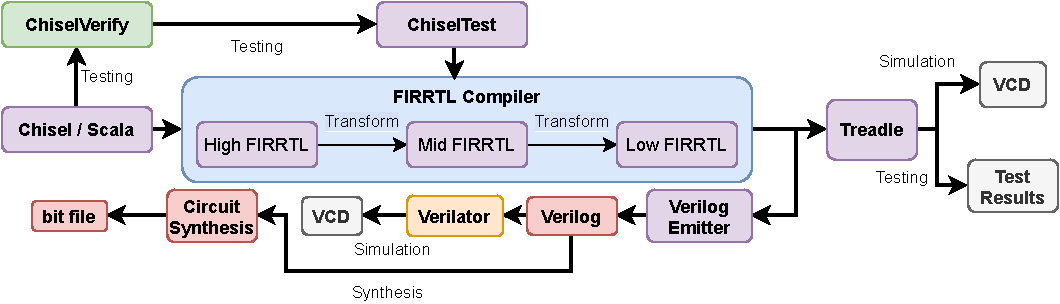
\includegraphics[width=0.8\linewidth]{Chisel_FIRRTL_VERILOG.pdf}
    \caption{Overview of the Chisel compilation pipeline.}
\label{fig:chisel-pipe}
\end{figure*}

\subsubsection{Constrained Random Verification}
Using constrained random verification features, a verification engineer can create random variables constrained to 
specified sets of values. In doing so, even a relatively small test suite can, statistically, 
cover many functionalities of a design. Moreover, constraining inputs ensures that no 
unnecessary tests are run for input combinations that would not appear during regular 
operation~\cite{MehtaCRV2018}.

A set of constrained random variables define a Constraint Satisfaction Problem (CSP). In CSPs, 
problem entities are represented as a finite, homogeneous collection of constraints. CSP solvers 
seek solutions to such problems and, thus, serve as the basis for constrained random verification.

Constrained random data types are native and declared with the \texttt{rand} keyword in SystemVerilog. 
Implementations of SystemVerilog simulators have a built-in CSP solver allowing for randomization through its \texttt{randomize} method.

\subsubsection{Bus Functional Models}
Abstraction is often the key to solve complex problems. Bus functional models represent such 
a technique. They implement models of (standardized) interfaces, like the Advanced eXtensible Interface version 4 (AXI4) from ARM~\cite{axi4standard}, that enable 
interacting with either master or servant components at a transaction level that abstracts away 
bit-fiddling of individual wires. Digital hardware vendors often provide IP generators whose output 
blocks are equipped with such interfaces. Well-developed bus functional models enable simpler, safer, and less 
verbose interactions with such components.

\subsection{The Chisel Hardware Construction Language}\label{subsec:chisel}

Chisel is a ``hardware construction language'' embedded in the general purpose programming language Scala~\cite{bachrach2012chisel, chisel:book}.
It allows designers to effectively write Scala programs that generate hardware descriptions at the Register Transfer Level (RTL).
Compared to traditional hardware description languages, like 
VHDL and Verilog, Chisel is much more high-level and allows for object-oriented and functional 
programming in the context of digital design.
One popular open-source application is the powerful RocketChip system on chip generator~\cite{rocketchip}.

The user-facing API of Chisel is a Scala library with some syntactic sugar that allows the user to generate RTL designs.
These designs then have to be converted into a format that is understood by simulators as well as FPGA and ASIC synthesis tools.
The lowering is done by the FIRRTL compiler which converts a high-level Intermediate Representation (IR) into a normalized structural representation~\cite{firrtl}.
The low-level representation is then exported into a subset of Verilog that was chosen as a common subset supported by the majority of backend tools.

Besides serving as a convenient way to lower Chisel circuits into Verilog, the FIRRTL IR and accompanying compiler infrastructure
also makes it easy to add circuit analysis and instrumentation passes, known as \textit{transforms}. Moreover, it is possible to simulate circuits described in FIRRTL using the Treadle execution engine, before converting them into (System)Verilog which can, of course, be simulated using commercial or open-source tools like Verilator~\cite{verilator}. Figure~\ref{fig:chisel-pipe} shows an overview of the Chisel compilation pipeline.

Being embedded in Scala, Chisel is executed on the Java virtual machine (JVM) and can
use existing Scala and Java libraries for design and verification. 
The JVM also allows for the use of the Java native interface for calling C functions, 
thus enabling co-simulation of Scala testers, Chisel designs, and a C-based golden models. This is 
valuable for companies wishing to keep their existing C models while using Scala/Chisel for simulation.

\subsection{Testing Chisel Designs}
A Chisel design can be tested with ChiselTest~\cite{chisel:tester2}, a non-synthesizable 
testing framework for Chisel that emphasizes simplicity while providing ways to scale up 
complexity. Like Chisel, ChiselTest is a Scala library that provides an interface into several 
simulators through \texttt{peek} (read value from circuit), \texttt{poke} (write value to 
circuit), and \texttt{step} (advance time) operations. Tests written with ChiselTest are just 
imperative Scala programs that run one line after another.

However, ChiselTest is missing fundamental functionalities that improve verification efficiency. 
For example, it does not provide either of the three aforementioned features: functional 
coverage, constrained random variables, or bus functional models, despite these features being 
crucial for efficient verification.

\section{Verification with Chisel}
\label{sec:verify}

As an extension of ChiselTest, we propose ChiselVerify, which introduces verification functionalities to the Chisel ecosystem.
ChiselVerify bases itself on ChiselTest by using its design interfacing features in order to enable various verification functionalities directly in Chisel, such as functional coverage, constrained random verification, and bus functional modeling. 
In the following subsections, we present how we achieved our solution.
We start by presenting its functional coverage capabilities,  using both implicit and explicit specifications.
We then propose constrained random verification tools for automating testing of general designs.
% , as well as a constrained program generation tool for verifying processors designed in Chisel. MS: not there (yet)
Finally, we look at how bus functional models can increase testing ease, and demonstrate our method by creating a model of the standardized AXI4 interface. 


\subsection{Coverage in Chisel}
% Proposed rewrite
ChiselVerify allows for functional coverage constructs to be defined over a Chisel design directly in Scala. 
This is possible directly inside of a ChiselTest test bench, and enables the gathering of information about completeness of a test with relation to a given specification defined using a verification plan.
In order to enable functional coverage in Chisel, we explore and define two methods for describing a specification, using an \emph{implicit} or an \emph{explicit} verification plan.
These two methods are defined as follows:

\begin{itemize}
	\item \textbf{Implicit verification plan:} Omit the verification plan, and obtain coverage data through queries on the ports we want to check \emph{after} the test bench.
	\item \textbf{Explicit verification plan:} Declare the ports that will be sampled \emph{before} the test bench.
\end{itemize}

Both methods have their advantages and disadvantages, which we will discuss in detail in a later section.
In both cases, in order to define our methods, we needed to be able to do the following:

\begin{itemize}
  \item Create a verification plan, either implicitly using a \texttt{Queryable} reporter, or explicitly using \texttt{cover} constructs, 
  \item sample our tested device's ports, using ChiselTest's interfacing capabilities, 
  \item keep track of the different sampled values that hit for each bin, using a coverage database, and 
  \item compile all of the results into a comprehensible and programmatically useful coverage report.
\end{itemize}

We will describe how the two different solutions are used to gather functional coverage information.

\paragraph{Implicit Verification Plans} As presented above, our solution enables the gathering of functional coverage information without explicitly having to define a specification.
This is enabled through the use of a \texttt{QueryableCoverage} object, which is simply defined on a given DUT.
The object must be defined within a ChiselTest test bench, allowing for the existence of a usable DUT.
Once that is done, it must be sampled throughout the test suite using its \texttt{sample} method.
Doing so will store the current value of every port in the DUT, thus enable for a future coverage queries.
Obtaining coverage information using this method is done at the end of a test suite using coverage queries of the form of \texttt{get(port, expectedHits, range)}, where the arguments have the following meaning:
\begin{itemize}
	\item \texttt{port} represents the DUT port for which we want coverage information.
	\item \texttt{expectedHits} is optional and represents a specification of number of hits we would expect for this port.
	\item \texttt{range} is also optional and represents the range in which we want to sample the port.
\end{itemize}
A query of this sort yields a \texttt{CoverageResult} case class that can then be used either programmatically or to generate a readable report using its \texttt{print} method.
One can also simply print out a full report of all ports in the DUT using the \texttt{QueryableCoverage} object's \texttt{printAll} method.

\begin{lstlisting}[captionpos=b,caption={Example use of Queryable coverage in order to gain information about the DUT's testing process. Note that \texttt{outA} and \texttt{outB} simply output the values of \texttt{a} and \texttt{b}.},label={lst:implcov},language=scala]
val coverage = new QueryableCoverage(dut)
for (fun <- 0 until 50) {
  dut.io.a.poke(toUInt(fun))
  dut.io.b.poke(toUInt(fun % 4))
  coverage.sample()
}
coverage.get(dut.io.outA, 50).print()
coverage.get(dut.io.outB).print()
coverage.get(dut.io.outA, range = 0 to 4).print()
coverage.printAll()
\end{lstlisting}
Listing~\ref{lst:implcov} shows a basic use of the implicit coverage tool. 
The above example outputs the following coverage Report:  
\begin{verbatim}
Port io_outA has 50 hits = 100.0% coverage.
Port io_outB has 4 hits.
Port io_outA for Range 0 to 4 has 5 hits 
= 100.0% coverage.  

========= COVERAGE REPORT ========= 
Port io_outAB has 26 hits.
Port io_outB has 4 hits.
Port io_outA has 50 hits.
Port io_b has 4 hits.
Port io_a has 50 hits.
===================================
\end{verbatim}
This report shows the coverage results from our simple test in the form of the number of hits associated to each port.
Given a specification for the amount of expected hits, the tool also shows a coverage percentage over the port.
We can also see that given a range, the tool is also able to output a coverage percentage using the range length as the expected number of hits.

Queryable coverage can be a useful tool for gathering simpler coverage information on a DUT.
However, in order to define complex specifications for our functional coverage, explicit verification plans must be used.

\paragraph{Explicit Verification Plans} As detailed in our previous work on the topic~\cite{dobisCoverage:ETS22}, our solution allows for the definition of a target specification using a set of \texttt{cover} constructs defined inside of a \texttt{CoverageReporter}.
This reporter functions as a front-end element that allows for the definition of complex specifications using only high-level constructs.
The main interface is the \texttt{register} method, which stores \texttt{cover} construct to \texttt{bin} mappings inside of a \texttt{CoverageDB} database object, and groups them as a single \texttt{covergroup}.
After the definition of the verification plan, the registered elements of the specification must be sampled explicitly by the user using the \texttt{sample} method, which checks the value of the associated port at that simulation cycle against the bins in order to determine if the specification is met for that value or not.
Once the sampling has been done, at the end of a test suite, a functional coverage report is generated by the reporter using the \texttt{report} method, which interprets the results stored in the database and compiles them to into a Scala \texttt{case class}. 
This report object can then be used to check for coverage thresholds, i.e., whether or not the coverage has surpassed a specific amount, or to guide the mutation of inputs in a mutation-based fuzzer, as was explored in previous work~\cite{verify:fuzzing:2021}.

\begin{lstlisting}[captionpos=b,caption={Small verification plan defined using 3 \texttt{cover} constructs, including one cross coverage construct},label={lst:basicfuncov},language=scala]
val cr = new CoverageReporter
cr.register(
  cover("accu", dut.io.accu)(
    bin("lo10", 0 to 9),
    bin("First100", 0 to 99)),
  cover("test", dut.io.test)(
    bin("testLo10", 0 to 9)),
  cover("accuAndTest", dut.io.accu, dut.io.test)(
    cross("both1", 1 to 1, 1 to 1))
\end{lstlisting}

Listing~\ref{lst:basicfuncov} shows a basic verification plan defined using our functional coverage tool. 
This example shows the use of \texttt{cover} constructs with both a single and multiple ports. 
The use of multiple ports defines a \textit{cross coverage} relation between the two ports, meaning that sampled values are considered a \emph{hit} if they meet all specifications simultaneously~\cite{spear2008systemverilog}.
Concretely, in our example, a hit would be considered if, within the same cycle, both \texttt{dut.io.accu} and \texttt{dut.io.test} are sampled with the value \texttt{1}. 

After defining our specification in the form of a verification plan, we need to define the ideal location, within our test bench, to sample the registered \texttt{cover} constructs using the reporter.
The reporter's \texttt{sample} method can be used to sample either all groups simultaneously or simply one group at a time, by specifying the \texttt{id} of the group we want to sample in the method call.
All \texttt{cover} constructs within a group will always be sampled together.
Sampling different groups at different locations throughout the test suite can allow for more targeted coverage information to be gathered.
Finally, once we are done sampling throughout the test suite, we can print out a readable coverage report by calling \texttt{cr.printReport()} which, for our example, results in the following: 

\begin{verbatim}
=============== COVERAGE REPORT ===============
================= GROUP ID: 1 =================
COVER_POINT PORT NAME: accu
BIN lo10 COVERING 0 to 9 HAS 8 HIT(S) = 80%
BIN First100 COVERING 0 to 99 HAS 9 HIT(S) = 9%
===============================================
COVER_POINT PORT NAME: test
BIN testLo10 COVERING 0 to 9 HAS 8 HIT(S) = 80%
===============================================
CROSS_POINT accuAndTest FOR POINTS accu AND test
BIN both1 COVERING 1 to 1 CROSS 1 to 1 HAS
1 HIT(S) = 100%
===============================================
\end{verbatim}

This report shows the three \texttt{cover} constructs that we registered and the associated hits that each of their \texttt{bins} has obtained.
These hits represent the number of times that registered port was sampled with a unique value found within the given range.
Each \texttt{bin} is then given a coverage percentage, based on the ratio between the number of hits obtained and the total number of possible values in the range.

In addition to the basic \texttt{cover} constructs presented until now, our tool allows for the definition of more complex relations, including delayed cross coverage, and purely conditional coverage.
Inspired by concepts from Linear Temporal Logic~\cite{Dax2010:temporal-logics}, delayed cross coverage allows the user to define a relation between two ports sampled at different clock cycles.
The idea is similar to how a \texttt{cross} works, but this time rather than sampling both points in the same clock cycle, we compare one port, at the starting clock cycle, to another port sampled a given number of clock cycles later. 
The temporal separation between the two ports is defined using a \texttt{delay}, for which we have defined four different types:
 \begin{itemize}
 \item \texttt{Exactly}, a hit is obtained if a value sampled from the second port meets its specification, as defined in the bin, exactly the given number of clock cycles after the first point was sampled.
 \item \texttt{Eventually}, a hit is obtained if the second port meets its specification at any point within the given number of clock cycles after the first point was sampled.  
 \item \texttt{Always}, a hit is obtained if the second port meets its specification at every clock cycle for a given number of clock cycles after the first point was sampled.
 \item \texttt{Never}, a hit is obtained if the second port never has a sampled value that meets its specification during any clock cycle for a given number of clock cycles after the first point was sampled.
\end{itemize} 
The use of timing-related bins is only possible if the coverage reporter is used to step the clock instead of ChiselTest's regular interface, since it allows for the \texttt{CoverageDB}'s internal clock to remain correct.

Conditional coverage enables the definition of bins containing fully custom hit-consideration rules using a user-defined predicate.
Using this type of construct, one can check for arbitrary relations between an arbitrary number of ports.
For example, it is possible to create a bin that checks for every clock cycle where all fields in a vector are equal.
This is done by using a function of type \texttt{Seq[BigInt] => Boolean} in the \texttt{bin} declaration.
The report then shows the number of distinct sampled values for which the predicate held throughout the testing process.
Given the unbounded nature of these bins, an ``expected number of hits'' argument is required for each condition in order to yield a final percentage alongside the number of hits.
Using these different types of \texttt{cover} constructs, one can express the specification of virtually any design.

\paragraph{Explicit vs. Implicit Verification Plans}
Comparing the two solutions, Explicit verification plans enable more precise and complex definitions of specifications than implicit verification plans.
This is due to the computational load inherently present in Implicit verification plans. 
Since Implicit verification plans require sampling over the entire range defined by the bit-width of every port, it is limited to use with simpler designs.
However, implicit verification plans do not require the re-simulation of a design in order to obtain different coverage information, while explicit verification plans do.
All in all, these coverage tools allow for the gathering of functional coverage directly in Chisel, thus filling in one of the holes inside of Chisel's ecosystem.
Another tool our solution brings to Chisel, and enables one of the uses of functional coverage presented earlier in this section~\cite{verify:fuzzing:2021}, is constrained random verification, which is detailed in the following paragraph.

\subsection{Constrained Random Verification}
%Proposed rewrite:
A coverage-driven verification suite is not complete without access to randomization tools.
ChiselVerify thus provides a set of tools, inspired by those available in SystemVerilog, which allow for the declaration and randomization of random objects.
This is done by providing a ``constraint programming" domain-specific language that runs on an existing CSP solver named JaCoP~\cite{jacop2013}.

\subsubsection{ChiselVerify's Constraint Programming DSL}
Our solution allows for the declaration of a constrained random object by defining a \texttt{class} that extends the \texttt{RandObj} trait.
The newly defined \texttt{RandObj} class contains all of the constraints and random variables that will later be used in our constrained random tests. 
This information will be stored inside of a \texttt{Model}, that is given to the \texttt{RandObj} on initialization.
In total, there are two main elements that are used inside of the object to drive the randomization process: random variables and constraints.

\paragraph{Random Variables} The first element represents a random value generator and is associated to constraints that will determine the set of values that the random variable can take.
Our DSL allows for the declaration of two different types of random variables: 
\begin{itemize}
	\item \emph{Regular}, can take any value that satisfies the associated constraints.
	\item \emph{Cyclic}, can not take the same values twice until the entire set of valid values has been explored.
\end{itemize}
Similar to the interface designed for the functional coverage tools, both types are declared using a single unified function call \texttt{rand} to which we give a lower and an upper bound on the values the variable can take.
As an example, \texttt{rand(0, 5, Cyclic)} will declare a random variable that will yield six distinct values in a row before starting to repeat itself.

\paragraph{Constraints} Our solution allows for the definition of both single constraints and \texttt{ConstraintGroup}s. 
Constraints are defined by applying constraint operators on random variables.
Additionally, the \texttt{IfCond} and \texttt{ElseC} constructs allow for the definition of conditional constraints.
Every defined constraint may be enabled or disabled at any point in the test suite. 
This can also be done to multiple constraints simultaneously by enabling or disabling a  \texttt{ConstraintGroup}.

\paragraph{Using a RandObj} After declaring and filling random objects with random variables and constraints, a \texttt{RandObj} must be instantiated and then randomized using the \texttt{randomize} method within a test bench.
The \texttt{randomize} method's return value is predicated on the solvability of the constraints by the CSP solver. 
Once randomized the random variables within a \texttt{RandObj} yield a valid random value when prompted with their respective \texttt{value()} methods.

\begin{lstlisting}[language=scala, caption={Example usage of a random object. \texttt{rand(min, max, type=Normal)} declares a random variable. Any operation on a random variable generates a constraint.}, label={lst:randobjscala}]    
class Packet extends RandObj(new Model(3)) {
  val idx = rand(0, 10)
  val size = rand(1, 100)
  val len = rand(1, 100)
  val payload: Array[Rand] = Array.tabulate(11)(
 	  rand(1, 100)
  )

  // Example Constraint with operations
  val single: Constraint = (payload(0) == (len - size))

  // Example conditional constraint
  val conditional = IfCon(len == 1) {
      payload.size == 3
  } ElseC {
      payload.size == 10
  }
  val idxConst = idx < payload.size
}
\end{lstlisting}

Listing~\ref{lst:randobjscala} shows an example use of the different ways one can define a random variable with constraints.
As seen in the example, collections of random variables, such as arrays, can be defined and constraints can be placed on the collections themselves.
This approach is seen in the \texttt{payload} random variable, where a constraint is placed on the size of an array of random variables.
The \texttt{conditional} random variable shows how conditional constraints can be declared.
In our example, the constraint placed on \texttt{payload} depends on the value of the \texttt{len} random variable. 

These constrained random objects are a powerful tool that can be combined with the aforementioned coverage functionalities to create coverage-driven randomized tests.
With the use of our solutions, such a setup greatly improves the automation capabilities of Chisel test benches.
However, these capabilities may be further improved by abstracting away groups of wires and operating on an operation or transaction level instead.

\subsection{Verification with Bus Functional Models}
Component re-use, portability and flexibility are also interesting in the context of digital 
designs. A good way to achieve these characteristics is by equipping one's designs with standardized 
interfaces. Verification engineers can test such components at a transaction level by combining constrained random verification 
and coverage measures with bus functional models. As an example, we provide a bus functional model for AXI4, an open standard by 
ARM~\cite{axi4standard}.

\subsubsection{Introduction to AXI4}
The AXI4 protocol by ARM is a generic, flexible interconnect standard. It comprises five independent handshake-based channels; three for write operations (\textit{Write Address}, \textit{Write Data}, and \textit{Write Response}) and two for read operations (\textit{Read Address} and \textit{Read Data}). Interconnect operations, known as transactions, consist of sequences of transfers across either set of channels. All channels share a common clock and reset.

As an example, consider a write transaction of 16 data elements. First, the manager provides the transaction attributes (e.g., target address and data size) as a transfer on the \textit{Write Address} channel. Next, it transfers the data elements one at a time over the \textit{Write Response} channel. Finally, the subordinate indicates transaction status on the \textit{Write Response} channel. Note that channel independence means that data may be transferred before the transaction attributes and that the read channels may operate at the same time~\cite{axi4standard}.

\subsubsection{Implementation}
To enable easy verification of AXI4-interfaced components using ChiselVerify, we provide definitions of channel wire bundles, abstract manager and subordinate classes, and a transaction-based bus functional model: the \texttt{FunctionalManager} class. Through parameterizing the manager with a \texttt{Subordinate} DUT provides a simple interface to control the DUT. Its two most important methods are \texttt{createWriteTrx} and \texttt{createReadTrx} to create and enqueue write and read transactions, respectively.

Our bus functional model implementation utilizes ChiselTest's multithreading features to allow for non-blocking calls to the aforementioned methods and for emulating the channel independence more closely. When a write transaction is enqueued and no other write transactions are in flight, the bus functional model spawns three new threads, one for each channel. The threads handle the bit-fiddling required to operate the channels.

\subsubsection{A Test Example}
Returning to the example of transferring 16 data elements, consider the test for a module called \texttt{Memory} listed below. First, a write transaction with 16 data elements takes just one call to \texttt{createWriteTrx} most of whose arguments have default values. It is equally simple to create a subsequent read transaction. Depending on the DUT implementation and due to channel independence, not waiting for a write to complete before initiating a read may return incorrect results.
\begin{lstlisting}[language=scala, caption={Using the AXI4 bus functional model with ChiselTest}, label={lst:axitest}]
class MemorySpec extends AnyFlatSpec with ChiselScalatestTester {
  behavior of "My memory module"
  it should "write and read" in {
    test(new Memory()) { dut =>
      val bfm = new FunctionalManager(dut)
      bfm.createWriteTrx(0, Seq.fill(16){0x7FFFFFFF}, 
        len = 15, size = 2)
      bfm.createReadTrx(0, len = 15, size = 2)
    }
  }
}
\end{lstlisting}

\subsection{Future Work}

In this paper our development stays mainly in the Chisel world and comparing it against UVM.
However, an interesting approach would be to mix and mach different approaches and tools.
The easiest combination is to use Chisel for the circuit description and UVM for verifiaction.
Chisel generates standard Verilog code that can be integrated with an UVM testing flow.
SystemVerilog components can also be integrated in Chisel as black boxes and we can
verify them with ChiselVerify on Verilator. However, the SystemVerilog code shall only
include Verilog code constructs that Verilator supports.

The most challenging approach would be to combine UVM and ChiselVerify. For example,
having an UVM test driver for the DTU, but using ChiselVerify with a golden reference
model written in Scala. We consider this interesting development question as future work.


\section{Formal Verification}
\label{sec:formal}
% introduce dynamic verification
% While working on the RTL level description of a new circuit, designers need to quickly test their design
% in order to iteratively improve it. Extensive testing is also a common requirement before sending a design to be
% fabricated as bugs discovered after ASIC fabrication can be costly or even impossible to fix.
% The most common approach to testing RTL is to write a test bench program that interacts with a simulation of the design.
% Errors are found through manual waveform inspection or assertions in the design or the test bench.

% explain bounded model checking
An alternative to exercising the circuit description with a set of concrete inputs is to symbolically explore the circuit execution
for any inputs for a limited number of cycles.
This technique is called bounded model checking~\cite{bmc} and works by unrolling the circuit for $k$ cycles and then asking a 
Boolean satisfiability~\cite{sat} or SMT~\cite{smt} solver whether there exists a set of inputs and starting states for the memories and registers in the
design, for which an assertion is violated.
If the solver returns a satisfying assignment to this query, we obtain a counter example that can be expressed as a test bench that
initialized the state to concrete values from the solver and then drives the inputs for $k$ cycles with the inputs obtained from the solver.
If the solver returns that there is no such assignment, we get a guarantee that our circuit will not hit any assertion violation for the first $k$
cycles of its execution.

\begin{figure}
    \centering
\begin{lstlisting}[language=scala]
class Quiz15 extends Module {
  /* [...] I/O definitions */
  val mem = SyncReadMem(256, UInt(32.W), WriteFirst)
  when(iWrite) { mem.write(iWAddr, iData) }
  oData := mem.read(iRAddr, iRead)

  when(past(iWrite && iRead &&
            iWAddr === iRAddr)) {
    verification.assert(oData === past(iData))
  }
}

class ZipCpuQuizzes extends AnyFlatSpec
  with ChiselScalatestTester with Formal {
  "Quiz15" should "pass with WriteFirst" in {
    verify(new Quiz15, Seq(BoundedCheck(5)))
  }
}
\end{lstlisting}

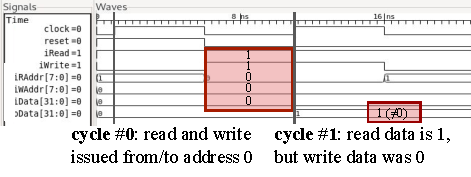
\includegraphics{woset_2021_quiz15.pdf}
\caption[Chisel verification example.]{This example verifies that when a Chisel memory with synchronous read port and
\code{WriteFirst} behavior has a read and a write access to the same address,
the new value will be returned.
The check fails if \code{WriteFirst} is substituted with \code{ReadFirst} or \code{Undefined} (Section~\ref{sec:undef}).
It is based on \href{https://zipcpu.com/answer/2021/07/03/fv-answer15.html}{a Verilog example from a popular blog}.
In the Chisel version, the assertion is automatically delayed until at least one cycle after reset, when there are valid \code{past} values available
(Section~\ref{sec:past}).
A bounded model check is executed by the \code{verify} command, which is called from a standard Scala unit test (Section~\ref{sec:flow}).
When the check fails, the failing inputs and starting states are replayed on a simulator, resulting in a waveform file that is identical
to the output we would get from a dynamic verification run.
However, since we used bounded model checking to find the failing trace, it will be as short as possible.
In our example, two cycles after reset are needed to fail the property.
The first cycle contains the read and write requests and the second cycle observes the arbitrary result on the read port if
we set the memory behavior to \code{Undefined} for read/write conflicts.
The included screenshot was obtained with the open-source GTKWave waveform viewer.
}
\label{fig:quiz15}
\end{figure}

\martin{The captions are too long. They should go into the main text.}

% the current state of the open-source ecosystem for formal verification
There has been a long tradition of open-source formal verification systems from the academic community~\cite{mcmillan1993smv, cimatti2000nusmv, mishchenko2007abc}.
% only citing select solvers for space gains
%~\cite{mann2021pono, mcmillan1993smv, cimatti2000nusmv, owre1996pvs, goel2020avr, vizel2014interpolating, mishchenko2007abc}.
However, because of the traditional academic incentive structure, these research systems were hard to use or did not support
enough features of the RTL design language to be widely used by a community of open source RTL designers.
This changed with the introduction of the yosys~\cite{Yosys} tool which has become the de facto standard for processing
Verilog for synthesis or formal verification.
Yosys allows academics to focus on developing model checkers for the simple btor2~\cite{btor2} or aiger~\cite{aiger} formats
without having to worry about supporting the much more complicated Verilog standard.
The open-source SymbiYosys~\cite{symbiyosys} tool wraps yosys as well as various formal verification engines in order to allow users to
verify their designs. All a user has to provide are the Verilog sources of their design including assertions and assumptions
as well as a small configuration script. SymbiYosys translates any failing traces it discovers into Verilog test benches and VCD waveform dumps
for the user to inspect~\footnote{With the open-source GHDL plugin, yosys now also supports formally verifying VHDL circuits.}.


% problems with the SymbiYosys approach
In this paper we describe our approach to providing Chisel users with an easy way to formally verify their designs.
We adapt many good ideas from yosys and build several new convenience features on top of them, taking advantage
of the existing compiler infrastructure for Chisel.

\subsection{Our Formal Verification Flow}\label{sec:flow}


Before we dive into some of the details of our implementation we want to present
the workflow that we imagine and illustrate how easy it can be to get started
with formal verification of a Chisel circuit~\footnote{
A scala project with executable examples as well as a Jupyter notebook are included in the companion repository to this paper:
\url{https://github.com/ekiwi/open-source-formal-verification-for-chisel}.
The contributions described in this paper are all part of the upstream \href{https://github.com/chipsalliance/firrtl}{firrtl}
and \href{https://github.com/ucb-bar/chisel-testers2}{chiseltest} libraries.
}.
The recommended way to start a Chisel project is to use the open-source Chisel template 
repository~\footnote{\url{https://github.com/freechipsproject/chisel-template}}.
The resulting Scala project automatically includes dependencies on the Chisel and the chiseltest
libraries which will be downloaded by the Scala build tool.

The template contains an example of using the chiseltest library to test a Greatest Common Denominator (GCD) circuit in simulation.
This test can be executed through a Scala IDE or from a shell with the \code{sbt test} command.
In order to turn this test into a formal check, we just need to substitute the \code{test(new DecoupledGcd(16))}
command with \code{verify(new DecoupledGcd(16)}, as well as provide the type of verification job as
\code{BoundedCheck(10)} and extend the testing class with the \code{Formal} trait.
If the user now clicks the test icon again or runs the \code{sbt test} command, a formal bounded check will
be executed for ten cycles after reset instead of a simulation test.
The only additional program required is a copy of the open-source SMT solver Z3~\cite{de2008z3}.

\begin{figure}[h]
\centering
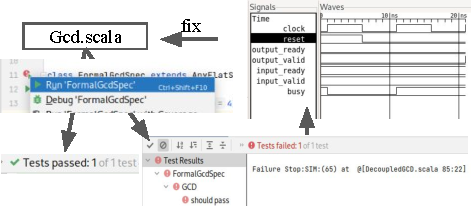
\includegraphics{woset_formal_ide_flow.pdf}
\caption{When working in a standard Scala IDE like the open-source IntelliJ IDEA with the Scala plugin, the user can launch the formal check with the press of a button.
The success or failure will be communicated the same way as any other unit test. A VCD waveform dump is automatically generated to help debug failing checks.}
\label{fig:ide-flow}
\end{figure}

Initially the check will always pass, no matter which changes we make to our circuit.
Since the GCD circuit contains no assertions, there is nothing to tell the solver if the circuits misbehaves.
In order to actually verify something, we can add assertions directly to the circuit by using the
Chisel \code{assert} statement.
The decoupled GCD circuit used as an example has an \code{input} and an \code{output} channel
as well as a 1-bit \code{busy} register.
We expect that while the circuit is busy, no new input is accepted:
\begin{verbatim}
when(busy) {
  verification.assert(!input.fire())
}
\end{verbatim}
This assertion will pass because the circuit does indeed fulfill the property after reset.


We now introduce a small bug by connecting \code{input.ready} to \code{true.B} and rerun the test.
An assertion violation will be reported one cycle after reset.
The user is also presented with an error message indicating the Scala line number of the failing assertion.
To debug the problem, they can find a VCD waveform dump in the standard test directory created by our
chiseltest library.
Since we replay the test on a concrete simulator, the error message and VCD will be exactly the same
as if the user was running a simulation test.
% Any improvements to our simulation interface or error reporting will thus immediately benefit formal verification
% users as well.

A more advanced property we expect to hold is that if the input and output channels are idle, the busy
signal will remain the same in the next cycle:
\begin{verbatim}
when(past(!input.fire() && !output.fire())) {
  verification.assert(stable(busy))
}
\end{verbatim}
Here we make use of our \code{past} function for temporal properties which is described in detail in Section~\ref{sec:past}.



\subsection{A Formal Backend for FIRRTL}\label{sec:undef}

\begin{figure}[h]
\centering
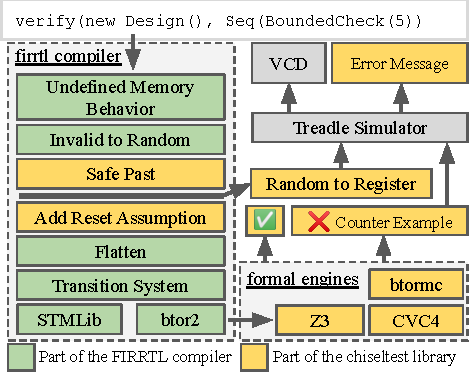
\includegraphics{woset_verify_flow.pdf}
\caption{The \code{verify} command is implemented as part of the chiseltest library and uses several compiler passes that make up the FIRRTL formal backend.
We hook into the FIRRTL compiler to model undefined behavior with \code{DefRandom} statements and to delay temporal assertions as part of our safe past construct.
We then add reset assumptions, flatten the system, convert to a formal transition system and then serialize the system to SMTLib or btor2.
We provide bindings to launch various formal engines from chiseltest.
If a counter example is found, we convert the \code{DefRandom} nodes in the circuit to registers before loading the circuit into the treadle simulator
to replay the failure and obtain a simulation quality VCD and error message.}
\label{fig:verify-flow}
\end{figure}

In order to implement the verify command, introduced in the previous section, we need to convert the Chisel circuit into a format that is understood
by open-source model checkers or SMT solvers.
We can do this by using the FIRRTL compiler to convert the circuit to Verilog and then using yosys to convert to the
model checking formats.
While we initially used this approach, we eventually decided that it would be better to add a formal backend to the FIRRTL
compiler directly.
This way we can avoid the complicated Verilog semantics, model circuit behavior in greater detail and easily replay counter
example traces on our FIRRTL simulator called treadle.

Users want their Chisel designs to be implemented with as little hardware as possible.
In order to allow for efficient implementations, the FIRRTL specification was crafted to allow
some operations to result in arbitrary results.
For example, a wire connected to \code{DontCare} or to the result of a division by zero carries an arbitrary value.
Reading from a memory while the read port is disabled, reading from the same address that another port is writing to or
writing from two memory ports to the same address all generate an arbitrary value result.
Not all of these behaviors are represented in the generated Verilog.
The compiler is free to substitute arbitrary values with (more) concrete values, like always returning a memory read result even
when the read port is disabled or by assigning a priority to write operations so that at least one of them will complete.
Thus if we first generate Verilog and then use yosys, we are only verifying one concrete translation of the design,
but there may be other legal translations that would violate the property.
This is relevant, e.g., in the context of memories when we use an external SRAM compiler that might try to
rely on the fact that write-write collisions can have arbitrary results in order to generate better hardware.
This is the reason why we decided to carefully model arbitrary values as part of the FIRRTL compiler's new formal backend.

Once the formal engine finds starting states and inputs that lead to an assertion violation, we need to help the user debug their design.
Since we do not have the large resources of a major EDA vendor, we would like to reuse as much of the existing simulator infrastructure as we can.
If we can replay the failing trace on our existing simulator, the VCD waveform dump and the error reporting will be of the same quality as
when writing a concrete test bench.
In order to be able to replay failures caused by arbitrary values, we carefully engineered two FIRRTL passes that analyze the circuit and
add wires to detect when a result is arbitrary as well as a mux to substitute the result with a connection to a \code{DefRandom} node in that case.
The new \code{DefRandom} construct provides a named arbitrary value that can change every clock cycle,
very much like a \code{anyseq} annotated wire in Verilog.
The formal backend implements \code{DefRandom} nodes as inputs that can be freely chosen by the formal engine.
To make \code{DefRandom} work with our simulator, we  replace the nodes with registers of the same type that are never updated by the hardware.
Instead we use the software interface to our simulator to update these registers with the values chosen by the formal engine in each cycle.
Figure~\ref{fig:verify-flow} shows our compilation flow in more detail.

The btor2 format does not support hierarchical circuits and we thus always flatten the system by inlining everything into a single module.
In order to ensure that we produce a good waveform dump, the counter example will be replayed on the non-inlined circuit.
We make use of the built-in annotation support of the FIRRTL compiler to automatically track name changes of all registers and memories in
the design as they are inlined. This way we can map initial states found by the formal engine back to their hierarchical names.

Once the circuit has been flattened, the conversion to a transition system is fairly straight forward.
We implemented a SMTLib and btor2 encoding that is very similar to the one pioneered by yosys.
We used the FIRRTL specification to accurately translate FIRRTL expressions to the bit-vector expression language defined by the SMTLib format~\cite{smtlib}.
Our backend supports memory and register initialization using the same user annotations as the Verilog backend.
Multi-clock support through a clock stuttering pass is work in progress, for now only circuits with a single clock domain are officially supported.

\begin{figure}[h]
  \centering
  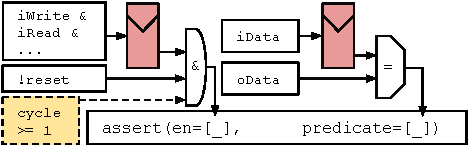
\includegraphics{woset_safe_past.pdf}
  \caption{The temporal assertion from Figure~\ref{fig:quiz15} results in a circuit with two registers created by the \code{past} function:
  One to delay the condition from the \code{when} statement and the other to delay the input data before it is compared to the current output data.
  By default an assertion is only enabled when reset is inactive and the surrounding \code{when} condition is true.
  Our compiler pass analyzes the connectivity graph with the result that both the enable condition as well as the predicate are delayed by a single past register.
  Thus the assertion enable signal is automatically extended to include the condition that at least 1 cycle must have past since the last reset.
  The new enable condition is derived from a synthesizable, saturating \code{cycle} counter which is created by the compiler pass.
  }
  \label{fig:past}
  \end{figure}
  

\subsection{Reset Assumptions}\label{sec:reset}

In Chisel, users rarely need to worry about resets.
Registers with reset values are automatically connected to the default reset % port of the module
and module instances just inherit their reset domain from their parent.
In Verilog, users have to manually ensure that assertions are only triggered after the circuit was properly reset.
We decided to provide sensible defaults instead.
Assertion statements are automatically disabled, just like it has been the case for print and stop statements
since the early days of Chisel.
As part of our formal verification support, we provide a FIRRTL pass
that automatically adds a constraint for the reset of the top level module to be active during the first cycle of execution.
Thus, by default, users do not have to worry about reset. Their assumptions will only fire
after their circuit has been properly reset and hence we ensure that there are no false positives.
We do provide options for power-users to write assertions that are active during reset and to
disable reset assumptions or increase the number of reset cycles.


\subsection{Simple Temporal Assertions}\label{sec:past}


While a simple \code{assert} statement allows us to specify a property over signals during a single
cycle, it is not enough to express properties that require us to reason about multiple cycles.
The traditional answer to this problem are temporal assertion languages like SystemVerilog Assertions~\cite{SystemVerilog}.
However, these are complex to implement efficiently and as of now there has not been a successful open-source implementation.
The community around SymbiYosys has instead advocated for the use of plain assertions with the Verilog \code{past}
function. This function returns the previous value of an expression and thus allows us to write properties that span multiple cycles.

While conceptually simple, the \code{past} construct as defined by the Verlog standard has one major problem:
In the first cycle of the circuit execution, there is no past value and the \code{past} function always returns X.
Thus the user has to take care to keep track of how many cycles have passed since the verification started and only enable assertions
once all past values are valid.
This particular pitfall is often the topic of a \href{http://zipcpu.com/quiz/2019/11/16/quiz07.html}{popular formal verification quiz}.
%In addition to that, \scalainline{past} values can also be invalid because they happened while
%the circuit was going through reset.

We made use of some of the unique capabilities offered by Chisel in order to implement what we consider to be a safer version of the
\code{past} function.
In the frontend, our \code{past} is a Scala function which creates an appropriate amount of delay registers in the current
clock and reset domain. That alone provides functionality similar to the Verilog version of \code{past}.
We go further by annotating the delay register and asking for a FIRRTL pass to be run when lowering the design.
This pass looks at a graph of all \code{past} delay registers and assertions in a module.
An edge indicates that the input to the assertion or register is connected to the output of a delay register through combinatorial logic.
We traverse the resulting tree (by design there can be no cycles) starting at each assertion
to find the longest path of \code{past} delay registers in order to determine the number of cycles the assertion needs to be delayed.
Finally we generate a cycle counter register and use its value to guard the individual assertions.
Since our \code{past} function only relies on synthesizable hardware it can also be used in software and FPGA based
simulation testing~\cite{karandikar2018firesim}.


\section{Evaluation}
\label{sec:eval}

In order to evaluate the different verification tools provided by ChiselVerify, we will be using three different example circuits, namely an accumulator ALU from the Leros processor~\cite{leros:arcs2019}, an arbiter circuit, and a priority queue provided by Microchip~\cite{microchip}.
These are tested using ChiselTest test benches augmented with our verification tools.
The test benches are then compared to similar tests written using SystemVerilog with UVM, and \texttt{cocotb}, using the generated Verilog descriptions as a DUT.
We have selected UVM since it is an industry standard that can be used to verify Verilog designs, and \texttt{cocotb} since it enables similar verification functionalities in a high-level environment like what we propose with ChiselVerify.
The results are then compared in terms of the verbosity of the verification code.
As a final evaluation, we look at the overhead induced by the use of ChiselVerify-specific functionalities, such as functional coverage and constrained random verification, by comparing the runtime of a bare ChiselTest test bench, to the same one enhanced with our verification tools.

\subsection{Evaluation Circuits}
We evaluate ChiselVerify on three distinct circuits, which we describe in the following paragraphs.

\subsubsection{Leros Accumulator ALU}

The first circuit we will verify with our solution is an accumulator ALU from the Leros processor.
It supports operations such as \texttt{add}, \texttt{load}, \texttt{shiftRight} and logic operations. 
In order to have a complete test suite, we need to try all available operations and use all potential input value corner cases.
We will thus model our test bench to do so.

\subsubsection{An Arbitration Circuit}

Another one of the circuits we evaluate ChiselVerify on is an arbiter circuit.
The arbiter uses a ready/valid interface for the clients and the shared resource. 
The arbiter is built as a binary tree, where each node does a local arbitration
and contains a register to store the data until it can be communicated further up towards the root of the
tree. Each local 2 to 1 arbiter has a turn flag to be fair between the two requests. The assumption is that
this local fairness translates to a global fairness of the full arbitration tree.

To test the arbiter, we specify properties that result in a verification plan:

\begin{itemize}
\item Each request shall eventually be seen at the output (the root node).
\item No requests shall be ``generated'' in the tree (out of thin air).
\item The maximum latency for a request shall be $n$ cycles without any competing requests.
\item The maximum latency for a request shall be $m$ cycles under full load.
\item The arbitration shall be fair, which means the bandwidth difference between clients shall be bound by $x$ \%.
\end{itemize}

The values of $n$, $m$, and $x$, depend on the number of clients, i.e., the size of the arbitration
circuit.

We have shown that the original implementation of \code{reduceTree} on the Chisel \code{Vec}
produces an unfair circuit. Therefore, we have improved that implementation in Chisel.
The pull request~\footnote{\url{https://github.com/chipsalliance/chisel3/pull/2318}} is now available
with Chisel Version 3.5.3.

\subsubsection{Sorting in Hardware}

%\martin{rewrite}

The final application example builds on a use-case provided
by Microchip~\cite{microchip}. The use-case, which we implemented and verified, is a scheduling module for real-time systems built around a hardware priority queue.
A host system can insert deadlines in the form of timestamps into the scheduling module which in turn presents the next upcoming deadline.

The scheduling module is implemented as a state machine 
operating on a set of memory banks. The memory contains a $k$-min-heap which is used by the internal priority queue to efficiently determine the next upcoming deadline. The implementation exploits parallelism to improve performance when fetching nodes from the heap memory by splitting siblings over separate memory banks. Furthermore, the search for the minimum key between a parent node and its children, a key operation when balancing the heap, can be parallelized by employing a reduction tree.

The presented constrained random verification and functional coverage functionalities of the ChiselVerify framework were used to verify the scheduling system and its submodules. 
The circuit at a top level allows for the insertion of deadlines into the scheduling system and the removal of them. As such the interface is not very complex and only consists of three flow-control pins as well as data pins used to provide a new deadline and to refer to a deadline which should be removed. 


%Due to the simple interface, which only consists of two flow-control inputs alongside the data fields, only distributional constraints were used to reduce the number of transactions marked as invalid. 
The test benches used to verify the scheduling system make use of random stimuli for the data pins and directed stimuli for the flow-control.
We use the functional coverage report to check how well the stimuli driven on the DUT's data pins are spread over the spectrum of possible values, and to check whether certain input combinations are applied to the DUT at some point throughout the test. 
As an example, the timed coverage feature made it easy to check whether the \texttt{valid} input of the DUT was revoked at some point within 10 clock cycles after issuing an operation by adding the following cross-coverage group:

\begin{lstlisting}[language=scala, caption={A timed cover construct.}, label={lst:timedcover}]
cover("timed_valid", dut.io.valid, dut.io.valid)(
  Eventually(10))(
    cross("revoked_valid_under_op", 1 to 1, 0 to 0))
\end{lstlisting}

In order to check whether the DUT matches its specification, we have implemented a reference model for each module. 
At the top level, this model is written at a transaction level, while some submodules are tested against cycle accurate reference models.
%As a reference model for the whole priority queue, a class was written which simulates state and interaction on a transaction/query level. 
In order to abstract interaction with the DUT and provide an interface at the same abstraction level as the reference model, we employ bus functional model-like wrappers. 
%These make it easy to think on a transaction or operation level when writing tests.

\subsection{Evaluation Results}
We can now take a look at the different results obtained during our evaluation.
\subsubsection{Verification Verbosity}
We start by comparing the three verification languages in terms verbosity, which is measured in ``verification lines per source lines of code'', a metric used in other works to partially evaluate verification languages~\cite{Nagini:2018, MuellerSchwerhoffSummers16, dobisCoverage:ETS22}.
We consider a verification line to be any explicit declaration of a cover or bin construct, as well as any function call or standard statement, and have formatted our listings accordingly.
For this, we measure the overhead of the functional coverage and constrained random verification tools provided in ChiselVerify against those provided in UVM and \texttt{cocotb}.

We start by adding functional coverage to the simple test bench presented for the arbiter circuit. 
In order to do so, we need to define a verification plan that correctly captures information about the expected behavior of our DUT.
The arbiter circuit takes as input a Vector of $n$ \texttt{DecoupledIO} elements, which expands to $3n$ ports in the generated verilog.
In order to conduct a coherent experiment, we set $n = 7$, and will define our specification accordingly.
Our verification plan will thus cover the inputs and output \texttt{ready}, \texttt{valid}, and \texttt{bits} (data) ports.

We now do the same for the priority queue. 
As described above, this design has two interfaces we will want to monitor during our testing, i.e.\ the \texttt{cmd} and \texttt{head} interfaces.
Unlike the arbiter, these interfaces are of fixed size and thus the chisel design and the generated Verilog will have similarly abstracted ports.
Our verification plan will thus cover all elements of both the \texttt{cmd} and \texttt{head} interfaces.
 
\paragraph{Functional Coverage in UVM} In order to gather functional coverage information about our design using UVM, we have to work with the generated Verilog description.
Additionally, UVM requires a very specific test bench structure than spans multiple files and hundreds of LOC.
Our focus is on the \texttt{uvm\_subscriber} subclass, which is where our verification plan will be defined.
For example, this is done for the arbiter circuit using the following structure:
\begin{itemize}
    \item Create a UVM-subscriber based coverage class.
    \item Instantiate the current DUT (\texttt{Arbiter dut = new;})
    \item Declare the verification plan, where a single port is covered with: 
    \begin{lstlisting}[language=verilog]
	covergroup cg_input0;
	IN0_READY: coverpoint dut.io_in_0_ready {
		bins zero = {0};
		bins one = {1};
		bins transitionzto 0 => 1;
		bins transitionotz 1 => 0;
	}
	IN0_VALID: coverpoint dut.io_in_0_valid {
		//Same bins as in IN0_READY
	}
	IN0_BITS: coverpoint dut.io_in_0_bits;
	endgroup cg_input0
	// [...] Repeat for each port
    \end{lstlisting}
    \item Define \texttt{build\_phase} and \texttt{write} functions.
    \item Define the coverage class constructor.
\end{itemize}  
Only considering coverage-related code, this requires 158 lines of SystemVerilog code. 

\paragraph{Functional Coverage in cocotb} Gathering functional coverage using cocotb is also done using the generated Verilog description.
This is done by creating a \texttt{Python}-based test bench, which is linked to our design via a custom \texttt{Makefile}.
We then define our verification plan by creating a \texttt{coverage\_section} inside of our test bench.
Finally, we link said verification plan to a \texttt{cocotb.coroutine} function to mark it as our sampler.
For example, the arbiter circuit's verification plan has the following structure:
 \begin{lstlisting}[language=Python]
 range_relation = lambda val_, bin_ : bin_[0] <= val_ <= bin_[1]
Arbiter_Coverage = coverage_section(
    CoverPoint("top.io_out_ready", vname="io_out_ready", rel = range_relation, 
        bins = [(0,1), 0, 1], bins_labels = ["ReadyStates", "ready0", "ready1"]),
    CoverPoint("top.io_out_valid", vname="top.io_out_valid", rel = range_relation, 
        bins = [(0,1), 0, 1], bins_labels = ["ValidStates", "valid0", "valid1"]),
    # [...] Repeat for each port
)
 \end{lstlisting}
 Only considering coverage-related code, this requires 82 lines of cocotb-coverage code.
 
\paragraph{Functional Coverage with ChiselVerify} Finally, using ChiselVerify to gather functional coverage information about a design allows for direct interaction with the Chisel design.
In the case of designs with complex interfaces, such as the arbiter, this allows us to create generic verification plans that function with any parametrization of the design.
For example, in the case of the arbiter, which has a variable number of inputs, we can simply define our verification plan using a generic loop over all inputs in the design as follows:
 \begin{lstlisting}[language=scala]
dut.io.in.foreach((input: DecoupledIO[UInt]) => {
  cr.register(
    cover(s"in${input.hashCode()}.ready", input.ready)(
        bin("ReadyStates", 0 to 1)),
    // [...] Continue the VP of a single input
  )
})
 \end{lstlisting}
Only considering coverage-related code, this definition requires 26 lines of code for the arbiter's complete verification plan.

\paragraph{Summary}
\begin{figure}[h]
  \centering
  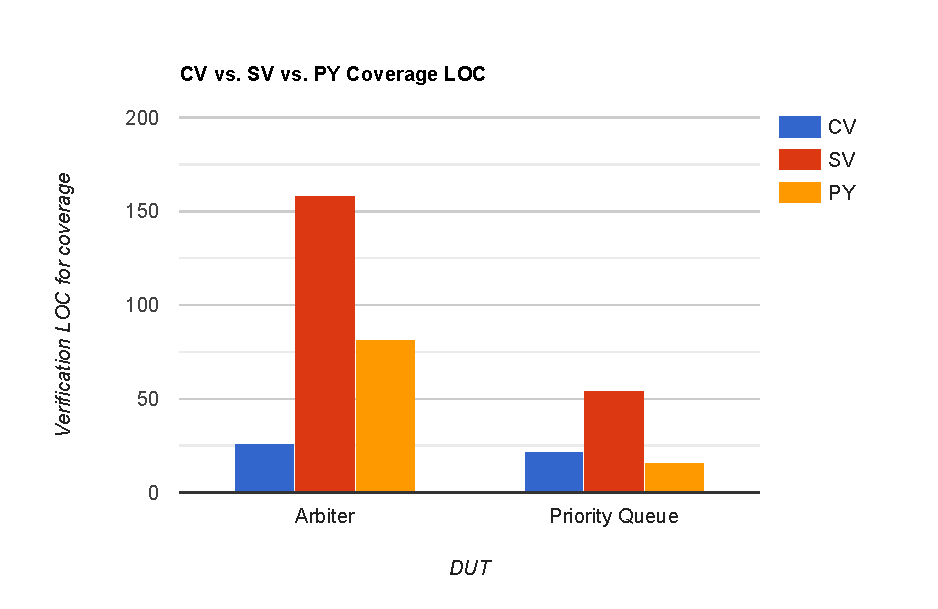
\includegraphics[trim=0.7cm 0.5cm 1cm 1cm, clip, width=.9\linewidth]{svcvpycomp.pdf}
  \caption{Verbosity overhead comparison between verification plans written for three designs with ChiselVerify (CV), SystemVerilog (SV), and cocotb (PY). For SV, only the \texttt{uvm\_subscriber} code is taken into account. }
  \label{fig:cvsvpycomp}
  \end{figure}
  
The results from our comparison are summarized in Figure~\ref{fig:cvsvpycomp}.
Figure~\ref{fig:cvsvpycomp} shows that, with ChiselVerify, we obtain on average a 70\% reduction in LOC over UVM and a 38\% reduction over cocotb. 
This is due to ChiselVerify's capability of exploiting the high-level design constructs, such as vectors, directly in the verification plan, while the other solutions need to rely on the unfolded generated Verilog.
For designs with simple interfaces such as the priority queue or the Leros ALU, we obtain an increase of 30\% over cocotb. 
This comes from cocotb's grouped bin declarations in a coverpoint.
However, this is an incomplete comparison, since cocotb does not provide the tools to express value transitions or temporal relations inside of a cover point, making its verification plan a less accurate model of our specification.
Thus, while it can be more concise to declare coverpoints in cocotb with simple designs, complex relations, often found in realistic designs, are more difficult to model.
It is much easier to access the ports from ChiselTest instead of UVM or cocotb, as we can use the original Chisel object.
This becomes especially important for deeper nested structures of IO ports.


\subsubsection{ChiselVerify Performance Overhead}
In order to evaluate our proposed solutions more thoroughly, we will look at the performance overhead that comes with using our verification tools to augment a ChiselTest test bench.
To do so, we use our baseline a bare ChiselTest test bench without any functional coverage or constrained random verification.

\paragraph{functional coverage Performance Overhead} In order to analyse the performance overhead over varying verification plan sizes, we will be using our previously mentioned arbiter circuit, which has a variable number of input ports.
We start by measuring the performance of our arbiter test bench with $n$ ranging from 2 to 256.
We then measure the performance of the same test bench, but this time augmented with the verification plan presented earlier.
Finally, we measure the performance of our initial test bench, but where the inputs of the arbiter are set using random variables from the following random object:
\begin{lstlisting}[language=scala]
class ArbiterIn(n: Int) extends RandObj {
  currentModel = new Model(seed)
  val dins = for(_ <- 0 until n) yield(rand(0, n))
  val consts = for(din <- dins) yield {
    din dist (
      0 to 0xF := 1,
      0xF to 0xFF := 1,
    )
  }
  // Enable all constraints
  consts.foreach(_.enable())
}
\end{lstlisting}
The results from these measurements are summarized in Figure~\ref{fig:cvoverhead}.
\begin{figure}[h]
  \centering
  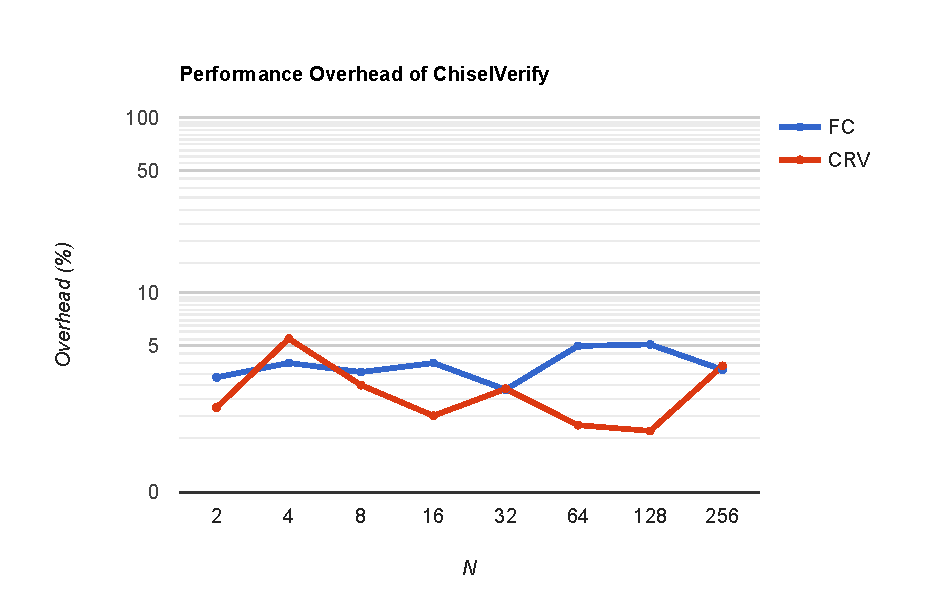
\includegraphics[trim=0.7cm 0.5cm 1cm 1cm, clip, width=.9\linewidth]{cvoverhead.pdf}
  \caption{Performance overhead of the different tools provided by ChiselVerify. N represents the number of arbiter ports which also means the number of covergroups or random variables. The overhead is computed as the ratio between the average runtimes, over many runs, of the bare ChiselTest test bench and the same test bench augmented with either functional coverage (FC) or constrained random verification (CRV) for a given $n$.}
  \label{fig:cvoverhead}
\end{figure}
These results show that the both the functional coverage and constrained random verification tools scale quite well, since their overheads seem to be almost independent of the size of the verification plan or the number of random variables used.
They both show to have an average overhead of 3.5\% over ChiselTest independent of the scale at which they are used.
Such a low and scalable overhead shows that ChiselVerify is an efficient addition to the Chisel verification ecosystem.

\subsubsection{Evaluation Summary}
As demonstrated above, ChiselVerify allows for the use of functional coverage constructs, as well constrained random verification directly inside of a ChiselTest test bench. 
Complex constructs can be defined following the low verbosity of Chisel and ChiselTest, requiring on average a 70\% fewer LOC than the industry standard UVM and a 38\% fewer than cocotb.
ChiselVerify improves upon these existing solutions by enabling direct use of high-level aspects of a Chisel design.
All of this is done with a low performance overhead, averaging at 3.5\% across the different functionalities.

\section{Conclusion}
\label{sec:conclude}

In this paper, we proposed well-integrated tools for verifying Chisel designs directly inside of a ChiselTest test bench. 
These include functional coverage and constrained random verification tools, as well as bus functional models all under a single library named ChiselVerify.
We also proposed formal verification methods, which are directly integrated into Chisel3, allowing for bounded model checking to be done in Chisel.
Using these tools on three different designs of varying complexity, we obtained similar results to those of using UVM or cocotb, all while requiring less verification code.
We also showed that the additional use of our tools within a ChiselTest test bench induces very little performance overhead.
With this, we enabled functional coverage, constrained random verification, bus functional models and formal verification techniques to be used in the Chisel/Scala ecosystem.
This will hopefully improve current verification engineering efficiency all while easing the way for software engineers to join the hardware verification world.

\subsection*{Source Access}

This work is in open source and hosted at GitHub:\\ \url{https://github.com/chiselverify/chiselverify}.
We plan also to regularly publish it on Maven.\footnote{https://mvnrepository.com/artifact/io.github.chiselverify/chiselverify}
The formal verification methods proposed in this work are integrated into Chisel3: \url{https://github.com/chipsalliance/chisel3}

%\subsection*{Acknowledgment}
%This work has been performed as part of the
%``InfinIT -- Innovationsnetv{\ae}rk for IT'', UFM case no. 1363-00036B,
%``High-Level Design and Verification of Digital Systems''.

\section*{Acknowledgment}
% feel free to cut the personal acknoledgements if desired:
We would like to express our thanks to the members of the Chisel community for their 
inspiration and help. % with making native formal verification for Chisel a reality.
In particular we are grateful to Tom Alcorn, Daniel Kasza, Jack Koenig, Deborah Soung,
Chick Markley, Schuyler Eldridge and Jiuyang Liu.
We would also like to thank Clair Wolf for all she has done to advance the open-source Verilog ecosystem.
Without yosys as an inspiration we would have never been able to conduct this work.
% the following founding acknoledgements need to stay in:
This work was supported in part by Semiconductor Research Corporation and through NSF grants CCF-1900968, CCF-1908870, and CNS-1817122.
Any opinions, findings, conclusions, or recommendations in this
paper are solely those of the authors and do not necessarily
reflect the position or the policy of the sponsors.


\bibliographystyle{IEEEtran}
\bibliography{../msbib,../chisel-uvm,kevin}%,../funding/ftp-chisel/testing}

\begin{IEEEbiography}[{
\includegraphics[trim={3cm 0 3cm 0}, width=1in,height=1.25in,clip,keepaspectratio]{bios/dobis.jpg}}]{Andrew Dobis}
is a Masters student in Computer Science at ETH Zurich. 
After obtaining his Bachelors degree in the same field from EPFL in 2020, he worked at the Technical University of Denmark (DTU)'s Embedded Systems Group as a Research Assistant.
His research focused on improving the verification capabilities of the Chisel Hardware Construction language, which lead to the creation of the ChiselVerify verification library.
His current research interests are more geared towards formal verification.
\end{IEEEbiography}

\begin{IEEEbiography}[{
\includegraphics[trim={1cm 0 1cm 0}, width=1in,height=1.25in,clip,keepaspectratio]{bios/kevin.jpg}}]{Kevin Laeufer}
  is a 5th year PhD Student in the ADEPT Lab at UC Berkeley.
  He is a major contributor to Chisel, in particular to the FIRRTL hardware compiler and the ChiselTest verification library.
\end{IEEEbiography}

\begin{IEEEbiography}[{
\includegraphics[width=1in,height=1.25in,clip,keepaspectratio]{bios/Hans.jpg}}]{Hans Jakob Damsgaard}
received the BSc degree in electrical engineering in 2019 and the MSc degree in
computer science and engineering in 2021 as part of the Honours programme at the
Technical University of Denmark, DTU. Currently, he is pursuing a PhD
on approximate reconfigurable accelerators for secure edge computing as part
of the APROPOS project at Tampere University. His research interests include
approximate hardware accelerators for neural networks, networks-on-chip, and computer architecture.
\end{IEEEbiography}

\begin{IEEEbiography}[{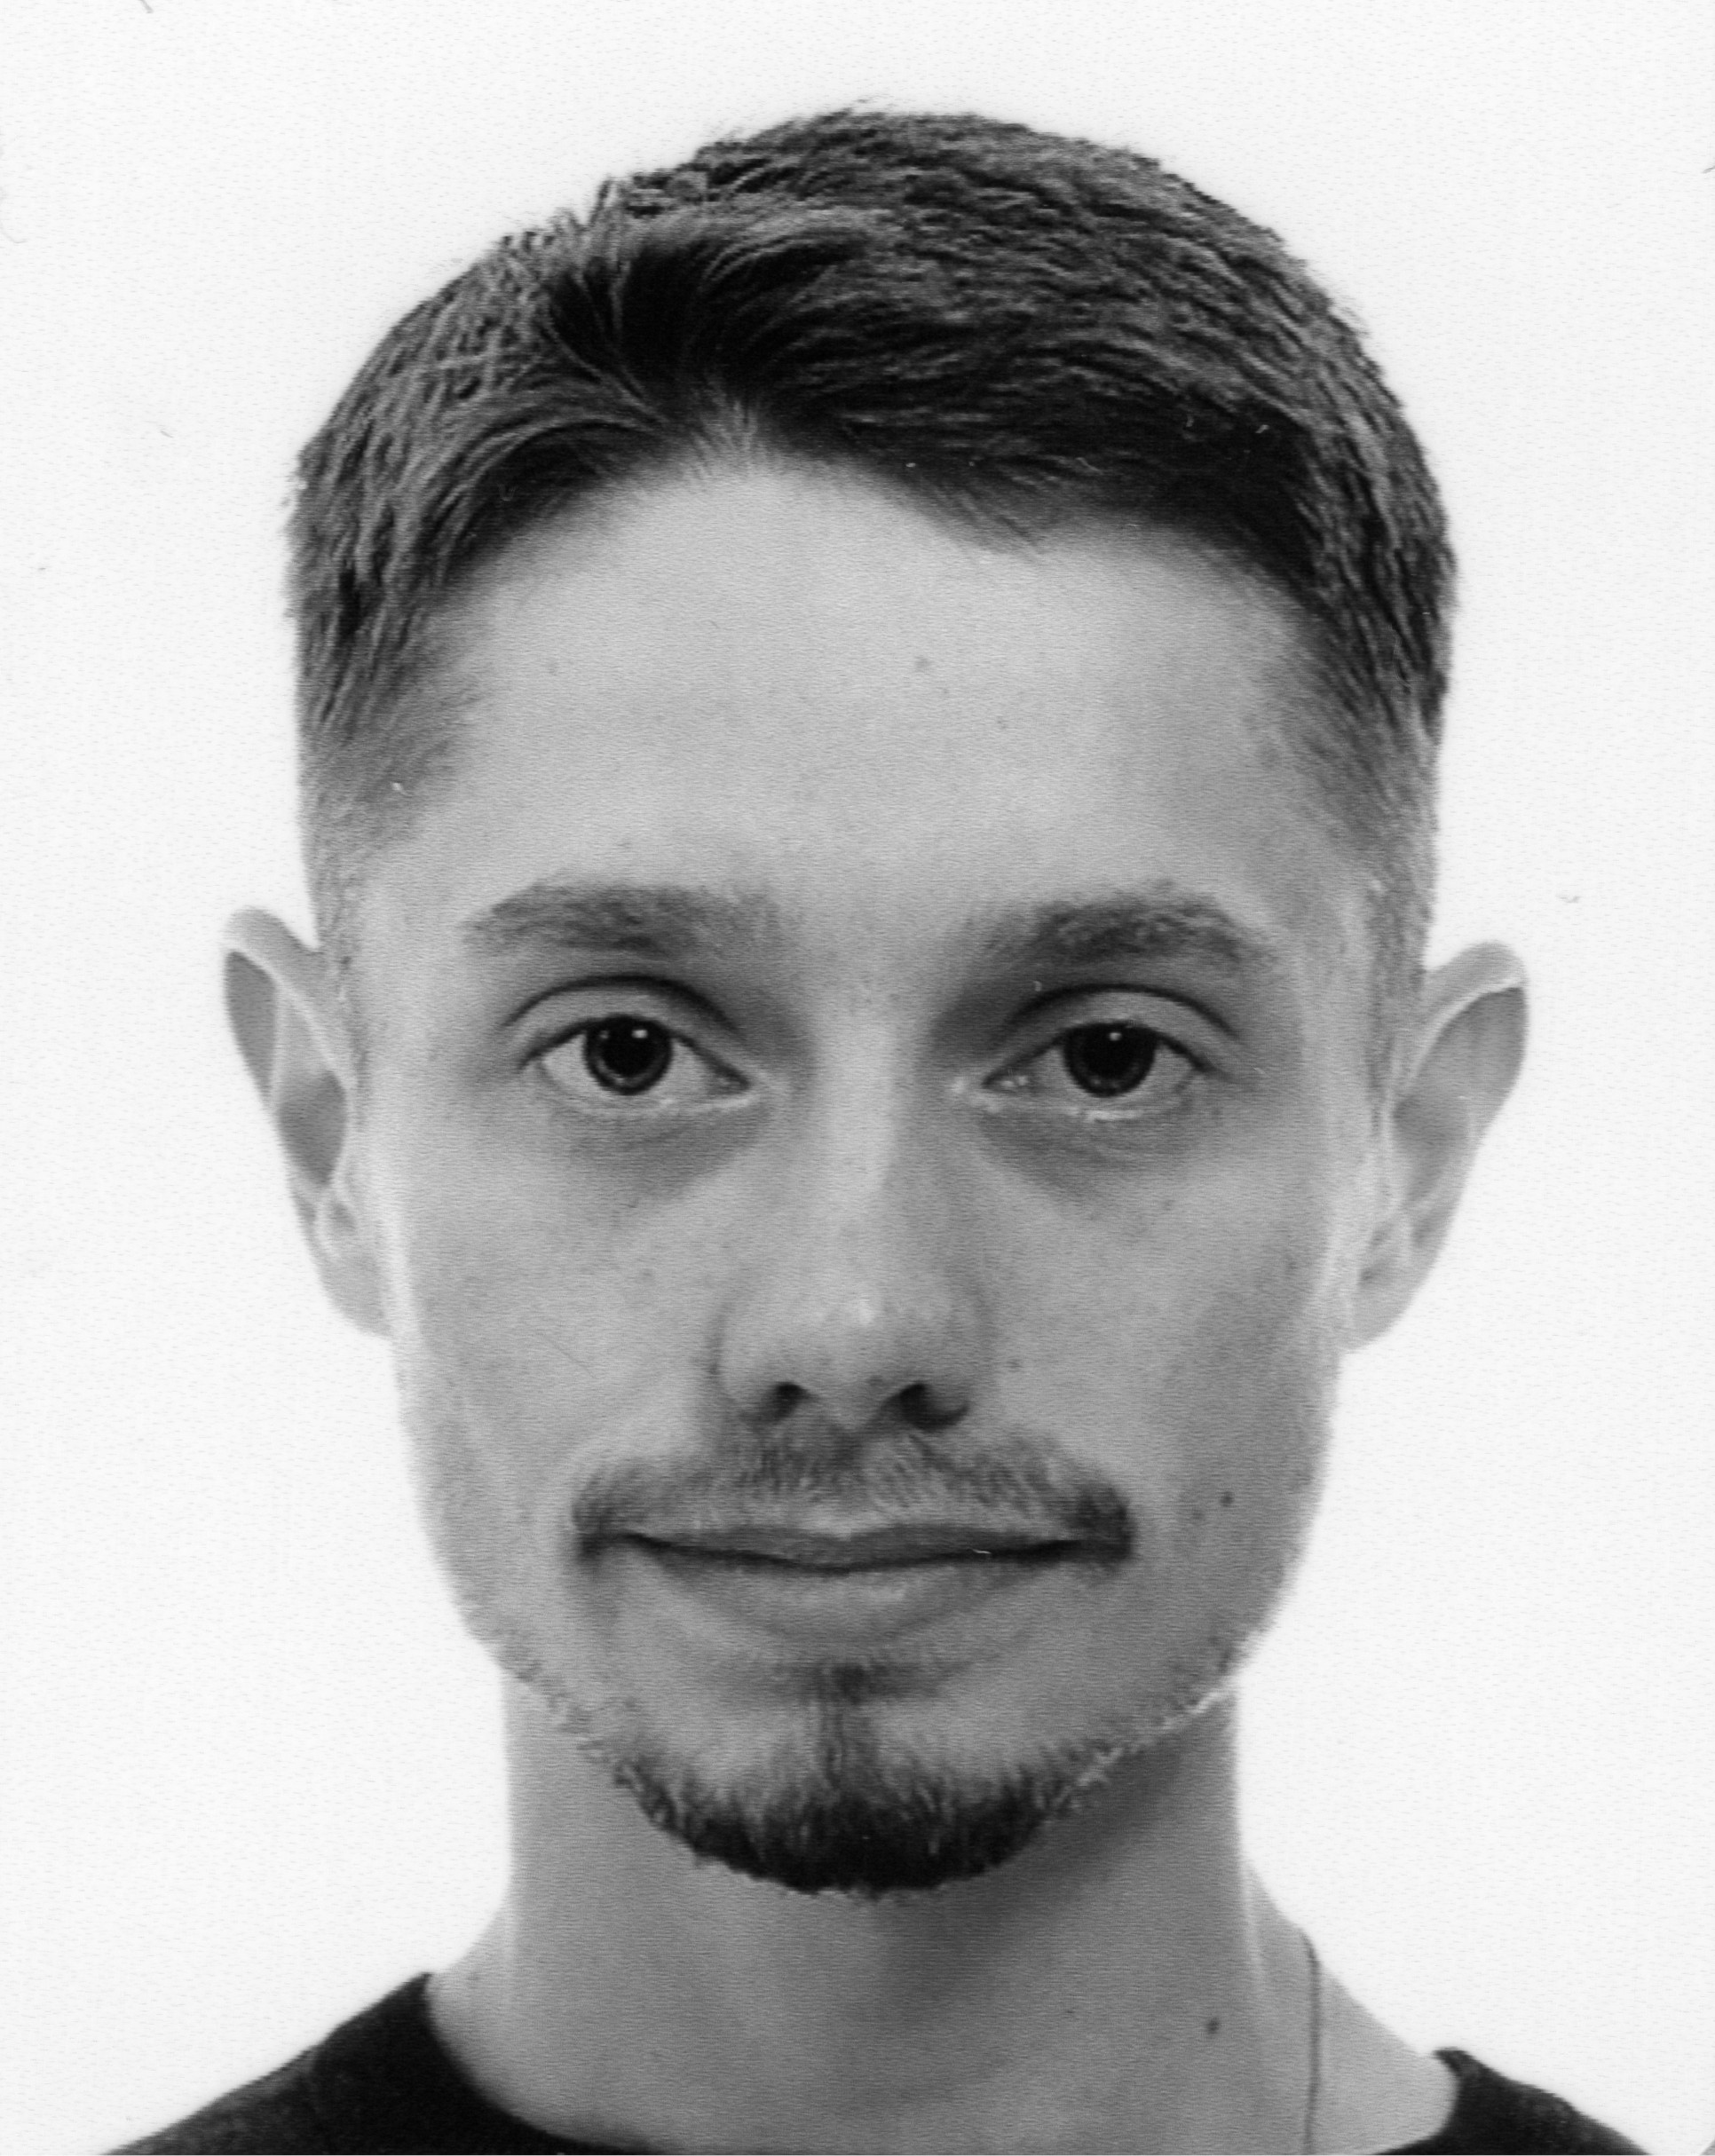
\includegraphics[width=1in,height=1.25in,clip,keepaspectratio]{bios/tjark.jpg}}]{Tjark Petersen}
  is a student at DTU in the final semester of the BSc in electrical engineering. 
  His research interest mainly revolves around digital design using Chisel, embedded systems and computer architecture.
\end{IEEEbiography}

\begin{IEEEbiography}[{
\includegraphics[trim={2.5cm 0 2.5cm 0}, width=1in,height=1.25in,clip,keepaspectratio]{bios/kasper.jpg}}]{Kasper Hesse}
  is a Masters student in Computer Science and Engineering at the Technical University of Denmark (DTU).
  His work at DTU's Embedded Systems Group was mainly on exploring UVM and C-Scala co-simulation using the JNI.
\end{IEEEbiography}

\begin{IEEEbiography}[{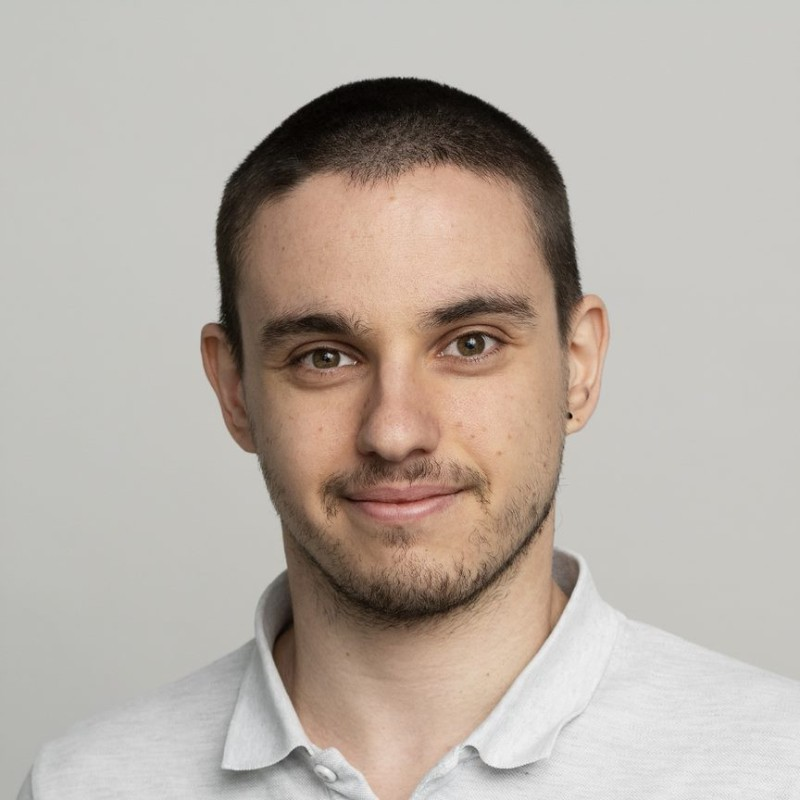
\includegraphics[trim={2.5cm 0 2.5cm 0}, width=1in,height=1.25in,clip,keepaspectratio]{bios/enrico.jpg}}]{Enrico Tolotto}
  obtained an MSc in Computer Science from the Technical University of Denmark in 2021.
  For his Masters thesis, Enrico worked on enabling constraint programming directly in Scala.
\end{IEEEbiography}

\begin{IEEEbiography}[{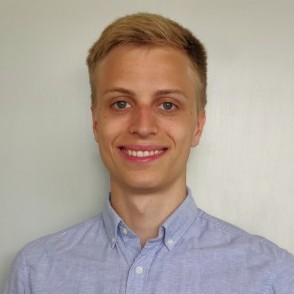
\includegraphics[trim={1cm 0 1cm 0},width=1in,height=1.25in,clip,keepaspectratio]{bios/simon.jpg}}]{Simon Thye Andersen}
  obtained an MSc in Computer Science from the Technical University of Denmark in 2020.
  After graduating, he worked on converting VHDL to Verilog code to enable the use of VHDL with Chisel testbenches.
  He now currently works at Teledyne RESON as a Firmware and Hardware engineer.
\end{IEEEbiography}

\begin{IEEEbiography}[{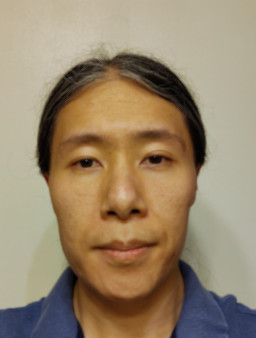
\includegraphics[width=1in,height=1.25in,clip,keepaspectratio]{bios/ducky.jpg}}]{Richard Lin}
obtained a PhD in Computer Science from UC Berkeley in 2021.  
His research focuses on open-source electronics design with a programming languages and human-computer interaction focus, and he is a major contributor to Chisel and the ChiselTest framework.
He is currently a post-doctoral researcher at UCLA.
\end{IEEEbiography}

\begin{IEEEbiography}[{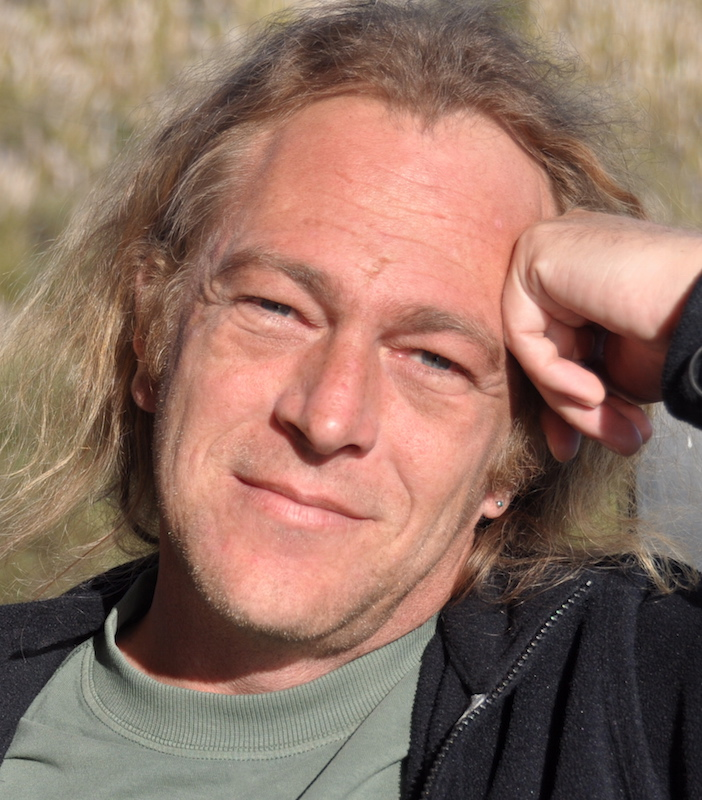
\includegraphics[width=1in,height=1.25in,clip,keepaspectratio]{bios/martin_small.jpg}}]{Martin Schoeberl}
  is Professor at the Technical University of Denmark (DTU), and has been since 2010.
  Before that, he was an Assistant Professor at the Institute of Computer Engineering at TU Vienna, where he had obtained his PhD in 2005.
  His research interests are mainly in Time-Predictable computer architecture, Real-Time systems, and more recently hardware verification.
  His work on time-predictable architectures lead to the EC funded project T-CREST (Time-predictable Multi-Core Architecture for Embedded Systems).
  He is also a contributor to Chisel, and has been teaching it in his digital design courses at DTU.
  He is the author of the only book on the topic, entitled ``Digital Design with Chisel".
\end{IEEEbiography}

\end{document}

%----------------------- REVIEW 1 ---------------------
%SUBMISSION: 222
%TITLE: ChiselVerify: An Open-Source Hardware Verification Library for Chisel and Scala
%AUTHORS: Andrew Dobis, Tjark Petersen, Kasper Hesse Rasmussen, Enrico Tolotto, Hans Damsgaard, Simon Thye Andersen, Richard Lin and Martin Schoeberl
%
%----------- Overall evaluation -----------
%SCORE: -1 (weak reject)
%----- TEXT:
%Summary: The paper describes a verification framework for Chisel. They demonstrate the framework on a priority queue.
%
%The abstract and introduction could use a major rewrite. Both cover quite a range of topics that are only tangential to their work. I suggest that they focus on making verification better for Chisel (the topic of their paper) rather than the end of moore's law, domain-specific acceleration and other tangentially related topics.
%
%"We can no longer depend on Moore’s Law to increase computing performance." I would be careful about such statements given that TSMC and Intel have just both announced continuations to their manufacturing processes for several more years. More importantly, is this really important to state in your abstract (which is quite long)? I would just focus on the problem that you are addressing.
%
%The same is true in the introduction. I would just remove the parts about domain specific. I just don't see them as all that relevant. Instead I would focus on the need verification for hardware designs. 
%
%"A few years ago, the two main design languages, Verilog and VHDL, dominated the design and testing of digital circuits." They still do (well, SystemVerilog).
%
%Section III.A can be reduced if needed for space. I feel it is ok to assume that the ICCD audience will know the basics of hardware test and verification.
%
%I feel Fig 2 is unnecessary. An ICCD reader will understand this.
%
%Once the paper got into the core of the materials, I found that it was well explained.
%
%Consider using the new ARM terminology Manager/Subordinate instead of Master/Slave. (see https://documentation-service.arm.com/static/604f31721da8f8344a2c9f18)
%
%The paper could use a more thorough evaluation of the tool. E.g., adding more examples/benchmarks and discussing the challenges and differences would significantly enhance the paper.
%
%++ The project is open-source!
%
%-- The link to the repo deanonymizes the paper. :(
%
%
%
%----------------------- REVIEW 2 ---------------------
%SUBMISSION: 222
%TITLE: ChiselVerify: An Open-Source Hardware Verification Library for Chisel and Scala
%AUTHORS: Andrew Dobis, Tjark Petersen, Kasper Hesse Rasmussen, Enrico Tolotto, Hans Damsgaard, Simon Thye Andersen, Richard Lin and Martin Schoeberl
%
%----------- Overall evaluation -----------
%SCORE: 1 (weak accept)
%----- TEXT:
%This paper presents the Open-Source Hardware Verification Library ChiselVerify. ChiselVerify is a part of the Chisel ecosystem. It has been developed with contemporary tools and languages. It supports features from UVM such as Constrained Random Verification or functional coverage but also adds features, such as Timed Cross Constraints. The paper compares it with currently existing solutions, such as SystemVerilog, UVM and other libraries in the Chisel universe. The paper also demonstrates the capabilities of ChiselVerify and explains its usage in a use case provided by an industry partner.
%
%The paper explains the features and thought processes behind ChiselVerify very well. Especially Sections 3 and 4 are well written. The goals behind ChiselVerify became clear and it is also demonstrated how it was achieved. The ideas behind ChiselVerify itself seem very thought out implementing existing practices and building additional features onto them such as time dependent cross conditions or conditional cover points where one can define an arbitrary condition.
%
%A small improvement would be to include ChiselTest and ChiselVerify in Figure 1 for a visual representation of how these libraries fit in the Chisel universe.
%There is also a typo in Section 1 in the fifth paragraph: "ChiselVerify is based _in_ the hardware [...]".
%
%There is a mention of a failed implementation of a CSP solver in Section 4, B in the first paragraph. This reads like a filler and should be removed.
%The paragraphs 4, 5 and 6 in the introduction feel disconnected and should be rewritten. A suggestion would be to move every mention of ChiselVerify into its own paragraph to give a rough idea of what ChiselVerify actually is.
%
%In the introduction the authors mention a comparison of Lines-of-Code between SystemVerilog and ChiselTest. It would have been interesting to mention how much more lines ChiselVerify is adding, since it seems that it builds on ChiselTest.
%The paper also mentions agile hardware development in the introduction and in the conclusion but it falls flat to handle that topic in the main part. The paper focuses on the design verification part, which is fine, but a few words about how ChiselVerify fits into the idea of agile hardware development would have been preferable.
%Section 5 feels superfluous. It does talk about how ChiselVerify was used in an industrial use case and describes said case and what has been done.
%But I do not see significant contribution to the paper in general that justifies this section. Section 4 and 5 could have been combined for example. Or another team implementing the same verification bench with UVM could have been employed and then the results compared. There is nothing measurable or comparable from the use case presentation.
%
%Overall, the paper has a well written description of ChiselVerify and how it fits into the Chisel universe.
%The Verification library itself seems thought out and the paper makes a good job of showing how ChiselVerify enriches the Chisel universe.
%But the paper also has its weaknesses. It did not pick up the topic of agile hardware development again. And there is Section 5 which does not really add anything meaningful to the overall contribution.
%There are some passages which feel like filler content, e.g., the failed implementation of a CSP solver.
%
%
%
%----------------------- REVIEW 3 ---------------------
%SUBMISSION: 222
%TITLE: ChiselVerify: An Open-Source Hardware Verification Library for Chisel and Scala
%AUTHORS: Andrew Dobis, Tjark Petersen, Kasper Hesse Rasmussen, Enrico Tolotto, Hans Damsgaard, Simon Thye Andersen, Richard Lin and Martin Schoeberl
%
%----------- Overall evaluation -----------
%SCORE: 2 (accept)
%----- TEXT:
%1. The link to the source code for ChiselVerify should have been made anonymous using http://anonymous.4open.science/ or another provider. Since the link is so clearly available in the paper and the authors are prominently mentioned on the GitHub repository, the authors are not really anonymous for this submission. This is a serious concern in terms of fairness to authors of other submissions. 
%
%2. This reviewer installed the code on Ubuntu and she/he was able to get the test examples up and running fairly easily. So, the library is readily available and usable.
%
%3. The results in the paper imply two contributions:
%(1) a well-integrated solution for verification of Chisel designs using a high-level language.
%(2) increase in productivity of the verification engineer
%The first contribution is clear and solid. However, the second contribution can only be established by conducting a study involving verification engineers that are not developers of this tool. That is missing from the paper.
%
%4. The algorithms presented in the paper are not very novel and the paper does not claim any such novelty. For example, the paper replaces their implementation of CSP Solving based on "Stuart Russel's book" by an existing implementation. As a minor point, the book has two authors; it is customary to refer to both authors if a book or paper has only two authors.
%
%In summary, this paper presents a tool that is publicly available and is likely to be useful.
%
%
%
%----------------------- REVIEW 4 ---------------------
%SUBMISSION: 222
%TITLE: ChiselVerify: An Open-Source Hardware Verification Library for Chisel and Scala
%AUTHORS: Andrew Dobis, Tjark Petersen, Kasper Hesse Rasmussen, Enrico Tolotto, Hans Damsgaard, Simon Thye Andersen, Richard Lin and Martin Schoeberl
%
%----------- Overall evaluation -----------
%SCORE: 0 (borderline paper)
%----- TEXT:
%This paper proposes a verification library for the hardware accelerators designed with Chisel and Scala.
%
%I can see a good amount of engineering efforts for chisel verification at a higher level than in Verilog. And the whole framework is open-sourced.
%
%However, the weakest part of the paper is the evaluation, which decreases the claimed benefits of the framework. The full evaluation is only showing with a simple sorting unit. This use case is too simple.
%
%It would be great to see the paper have a larger design case and a more complex setting with this amount of work. Also, the evaluation does not include the improvements, either in time or the efficiency of the proposed framework over the existing verification methods.
%
%
%
%----------------------- REVIEW 5 ---------------------
%SUBMISSION: 222
%TITLE: ChiselVerify: An Open-Source Hardware Verification Library for Chisel and Scala
%AUTHORS: Andrew Dobis, Tjark Petersen, Kasper Hesse Rasmussen, Enrico Tolotto, Hans Damsgaard, Simon Thye Andersen, Richard Lin and Martin Schoeberl
%
%----------- Overall evaluation -----------
%SCORE: -1 (weak reject)
%----- TEXT:
%The main purpose of this paper is to present a new way of verifying hardware designs with a proposed open-source library called ChiselVerify. The paper also provides background information and evidence of why it seems that digital design is the up-and-coming state of art and why we need better tools for it to be more efficient. It also provides a detail of how the library was designed and then used in a use case study provided by Microchip.
%Strengths:
%+The paper provides a good background of why it is important to invest time into digital design verification and seeks to provide a solution to help facilitate towards that direction. The flow and structure of the paper is easy to follow and does not cause confusion. 
%+The paper also provides a use case of the proposed library to show that it is effective for real industry use.
%Reviewer suggestions and Weaknesses:
%- One thing holding the paper back and making it a weak success is the lack of quantitative evidence when it claims the proposed library increases productivity. A comparison using other standard methods to perform the use case could offer some more clear advantages, even saying why the authors couldn’t use other methods for the use case would help with the productivity claim. Another thing that could be added is a table that clearly states which methods are able to preform the verification processes outlined in section III (i.e. functional coverage, constrained random verification, and bus functional models.)
%Comments for author
%- While the claim about Moore’s Law is a strong hook in the introduction, there really isn’t that much else provided to back that claim up. As is, if it and its citation source removed the paper loses no information and is not really changed significantly.
